\chapter{Synthesis: Comparing Temporal Dynamics and Spatial Topology}
\label{chap:synthesis}

\section{Introduction}
\label{sec:ch7_intro}

This chapter compares two families of derived summaries: per-channel reservoir dynamics (Chapter~\ref{chap:dynamics}) and graph topology (Chapter~\ref{chap:arspi_net}). Their electrode-wise association is called coupling. Because both families are transformations of the same trial-averaged EEG epoch, association does not establish a common latent neural mechanism or independence from shared preprocessing.

Chapter~\ref{chap:dynamics} reported condition-associated dynamical summaries, and Chapter~\ref{chap:arspi_net} reported descriptive graph summaries and exploratory clinical comparisons. The strongest nominal SUD comparison had parametric $p=0.0004$, but its label-permutation result was $p=0.073$. These results motivate a cross-summary analysis; they do not establish that one family uniquely represents condition and the other uniquely represents persons.

Related neuroimaging work examines relationships between local functional properties and network topology \cite{Deco2015,honey_network_2007,suarez_linking_2020}. Here $\kappa$ is only a norm of 14 within-epoch, cross-electrode rank correlations. It summarizes association among the derived quantities and has no direction, physiological unit, or demonstrated clinical utility.

The chapter reports archived four-category analyses (Threat, Mutilation, Cute, Erotic) and a separate three-condition analysis (Negative, Neutral, Pleasant). These are not replications: the input grouping, preprocessing, and archived reservoir implementations differ. In particular, the original four-category script omitted the post-spike threshold subtraction and nonnegative floor used by the three-condition pipeline. The audited script now uses the common update, but raw four-category EEG was unavailable for regeneration. Cross-analysis numerical differences are therefore descriptive and cannot be attributed to granularity alone.

Five exploratory analyses compare observed coupling with an electrode-permutation null, decompose sample sums of squares, inspect category differences, compare diagnosis-defined groups, and evaluate linear readouts built from the two descriptor families.


\section{Mathematical Framework}
\label{sec:ch7_framework}

\subsection{Data Objects}

For each subject $s \in \{1,\ldots,211\}$ and category $c \in \{\text{Threat, Mutilation, Cute, Erotic}\}$, two per-electrode descriptor matrices are constructed from the same $1229 \times 34$ category-level trial-averaged EEG epoch.

The \textbf{dynamical profile matrix} $\mathbf{D}_{s,c}\in\mathbb{R}^{34\times7}$ contains total spikes, mean firing rate, rate entropy, rate variance, temporal sparsity, permutation entropy~$\hat{H}_\pi$, and autocorrelation decay~$\tau_{AC}$ for each channel. These are descriptive metrics selected in Chapter~\ref{chap:dynamics}. Each column is computed after driving a fixed reservoir ($N_{res}=256$, $\beta=0.05$, $M_{th}=0.5$, seed~42) with a z-scored single-channel epoch. The archived four-category numbers were generated with the legacy reset update disclosed above.

The \textbf{topological profile matrix} $\mathbf{T}_{s,c} \in \mathbb{R}^{34 \times 2}$ contains two primary graph metrics for each electrode: weighted node strength and weighted clustering coefficient (Onnela formula) \cite{onnela_intensity_2005}. These are extracted from a $34 \times 34$ theta-band ($4$--$8$~Hz) time-averaged phase concentration (tPLV) matrix \cite{lachaux_measuring_1999}. Because the available data are category-level trial averages (one epoch per subject per category), the tPLV is computed as within-epoch phase concentration,
\begin{equation}
\label{eq:tplv}
\text{tPLV}_{ij} = \left|\frac{1}{T}\sum_{t=1}^{T} e^{j(\phi_i(t) - \phi_j(t))}\right|,
\end{equation}
where $\phi_i(t)$ is the instantaneous phase of the theta-filtered signal at channel~$i$. This is not classical trial-to-trial phase locking; it is within-epoch phase-difference concentration. Weighted strength and Onnela clustering are used as two summaries of the resulting dense weighted matrix \cite{rubinov_complex_2010}. Their reliability was not estimated here, and the unlabeled channel montage prevents anatomical interpretation.

\subsection{Coupling Measures}

The within-subject coupling matrix is defined by electrode-wise Spearman rank correlations between the two descriptor families:
\begin{equation}
\label{eq:coupling_C}
\mathbf{C}_{s,c} \in \mathbb{R}^{7 \times 2}, \quad (\mathbf{C}_{s,c})_{jk} = \rho_S(\mathbf{D}_{s,c}[:,j],\;\mathbf{T}_{s,c}[:,k]),
\end{equation}
where $\rho_S$ denotes Spearman correlation computed across the 34 electrodes. Each entry of $\mathbf{C}_{s,c}$ quantifies how one dynamical metric covaries with one topological metric across the electrode array for a specific subject and category.

The scalar coupling strength is the normalized Frobenius norm:
\begin{equation}
\label{eq:kappa}
\kappa_{s,c} = \frac{\|\mathbf{C}_{s,c}\|_F}{\sqrt{p \cdot q}} = \frac{1}{\sqrt{14}}\sqrt{\sum_{j=1}^{7}\sum_{k=1}^{2}(\mathbf{C}_{s,c})_{jk}^2}.
\end{equation}
This normalization maps $\kappa$ to $[0,1]$ and enables comparison across configurations with different $p$ and $q$. A $\kappa$ near zero indicates that the dynamical and topological descriptor families are unaligned across electrodes; a $\kappa$ near one indicates that every dynamical metric is strongly rank-correlated with every topological metric.

Spearman $\mathbf{C}_{s,c}$ and scalar $\kappa_{s,c}$ are the primary coupling instruments throughout this chapter. Canonical Correlation Analysis (CCA) is available as a secondary multivariate summary but is not used for primary inference due to the modest ratio of electrodes ($N_c = 34$) to variables ($p + q = 9$), which produces upward-biased canonical correlations in small samples \cite{wang_cca_2020}.

\subsection{Null Model}

The channel-permutation null shuffles the row indices of $\mathbf{T}_{s,c}$ relative to $\mathbf{D}_{s,c}$, breaking channel correspondence while preserving marginal values. For each of 5,000 permutations~$\pi$, a null coupling $\kappa_{s,c}^{(\pi)}$ is computed. The per-observation Monte Carlo $p$-value is
\begin{equation}
p_{s,c} = \frac{1 + \#\{\kappa_{s,c}^{(\pi)} \ge \kappa_{s,c}\}}{1 + 5000}.
\end{equation}
This null treats channel labels as exchangeable. Spatial smoothness and shared-reference effects can violate that assumption, so the result tests this particular label-shuffling null rather than a general null of no neurophysiological coupling.


\section{Data and Experimental Protocol}
\label{sec:ch7_protocol}

All experiments use the Stress, Health, and the Psychophysiology of Emotion (SHAPE) Community dataset \cite{noauthor_shape_2018}: $N = 211$ subjects (excluding subject~127), four IAPS subcategories (Threat, Mutilation, Cute, Erotic), yielding 844 subject--category observations. Each observation is a $1229 \times 34$ category-level trial-averaged EEG epoch at 1024~Hz, consistent with the data format in Chapters~\ref{chap:dynamics} and~5.

For each observation, the reservoir processes all 34 channels independently (28,696 total reservoir runs across the dataset). The tPLV matrix is computed from the same 34-channel epoch via theta-band filtering (3rd-order Butterworth, $4$--$8$~Hz) and Hilbert-transform phase extraction. Complete data for the five primary diagnoses are available for 206 of 211 subjects; 22 of those 206 are negative for all five (MDD, PTSD, SUD, GAD, and ADHD). The value 27 results only if the five incomplete records are incorrectly treated as diagnosis-negative and is not used. The supplied full-panel comorbidity variable has mean 2.8 (rounded) across 211 records.

Analyses use Wilcoxon signed-rank for paired summaries, Mann--Whitney~$U$ for group comparisons, and selected permutation tests. Bonferroni correction is applied only within explicitly stated families. Repeated categories from the same subject are not independent; where a test uses all subject--category rows without clustering or subject-level reduction, its $p$-value is labeled anti-conservative and descriptive.


\section{Experiment 7.1: Coupling Existence}
\label{sec:exp7_coupling}

\subsection{Mathematical Motivation}

Both $\mathbf{D}_{s,c}$ and $\mathbf{T}_{s,c}$ are derived from the same underlying EEG epoch through different transformations: the reservoir maps each channel's temporal signal into a dynamical descriptor, while the tPLV maps all pairwise phase relationships into a topological descriptor. If an electrode that participates in strong phase-locked interactions also drives the reservoir into a distinctive dynamical regime, then $\mathbf{D}_{s,c}$ and $\mathbf{T}_{s,c}$ will be rank-correlated across the electrode array. The observable quantities are the $7 \times 2$ coupling matrix $\mathbf{C}_{s,c}$, the scalar $\kappa_{s,c}$, and their distribution across 844 observations relative to the electrode-permutation null.

\subsection{Experimental Design}

For each of 844 subject--category observations, $\mathbf{C}_{s,c}$ and $\kappa_{s,c}$ are compared with 5,000 channel permutations. The archived group test applies a one-sided Wilcoxon test to all 844 differences between observed $\kappa$ and its null median. Because four rows come from each subject, that extremely small $p$-value is anti-conservative. An archived subject-level test compared mean $\kappa$ with zero; because $\kappa$ is a nonnegative norm with a positive finite-sample null expectation, that is not a valid confirmatory null test. A valid subject-level reanalysis would average $\kappa_{\mathrm{obs}}-\kappa_{\mathrm{null}}$ within subject or permute channel correspondence jointly within subject. The source package does not contain the raw inputs needed to regenerate the corrected four-category results.

\subsection{Raw Observation}

\begin{figure}[htbp]
\centering
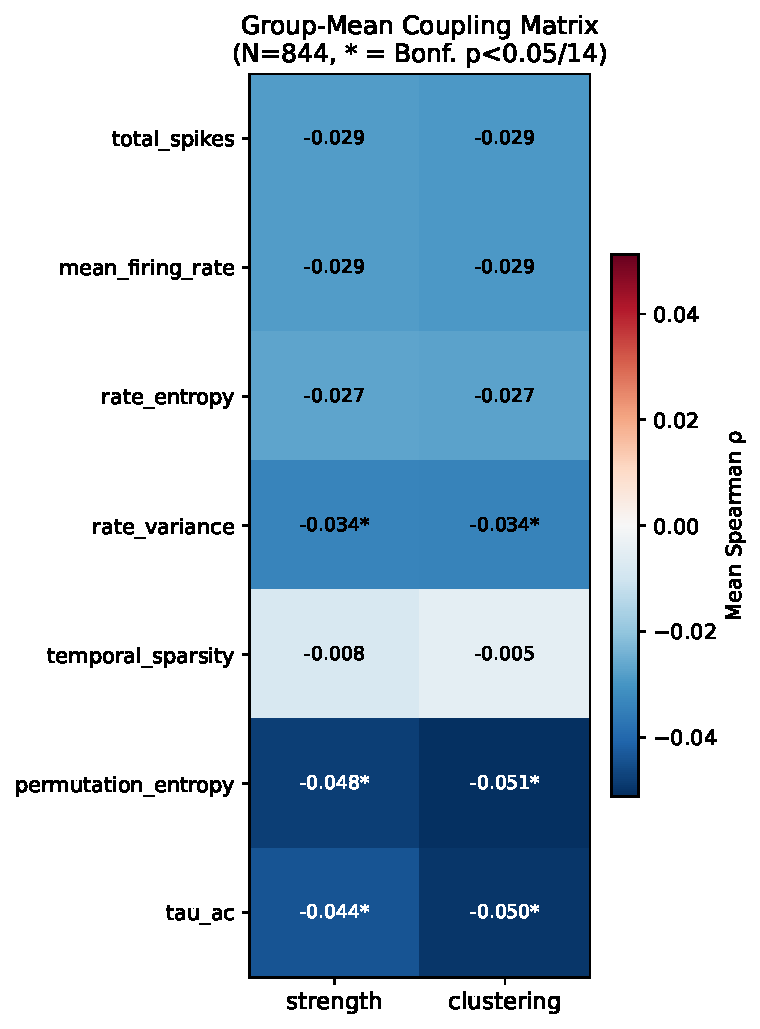
\includegraphics[width=0.65\textwidth]{pictures/chSynthesis/fig7_A1_mean_coupling_matrix.pdf}
\caption{Mean signed coupling matrix across 844 subject--category observations (211 subjects, four categories). All 14 sample means are negative. Asterisks reproduce archived Bonferroni-adjusted row-level tests, but those tests treat repeated categories as independent and are therefore descriptive.}
\label{fig:mean_C}
\end{figure}

All 14 sample-mean correlations are negative, ranging from $-0.005$ to $-0.051$ (Figure~\ref{fig:mean_C}). These are small cross-channel associations. They do not show that greater phase concentration causes a change in reservoir dynamics, and averaging conceals the mixed signs observed in individual matrices.

\begin{figure}[htbp]
\centering
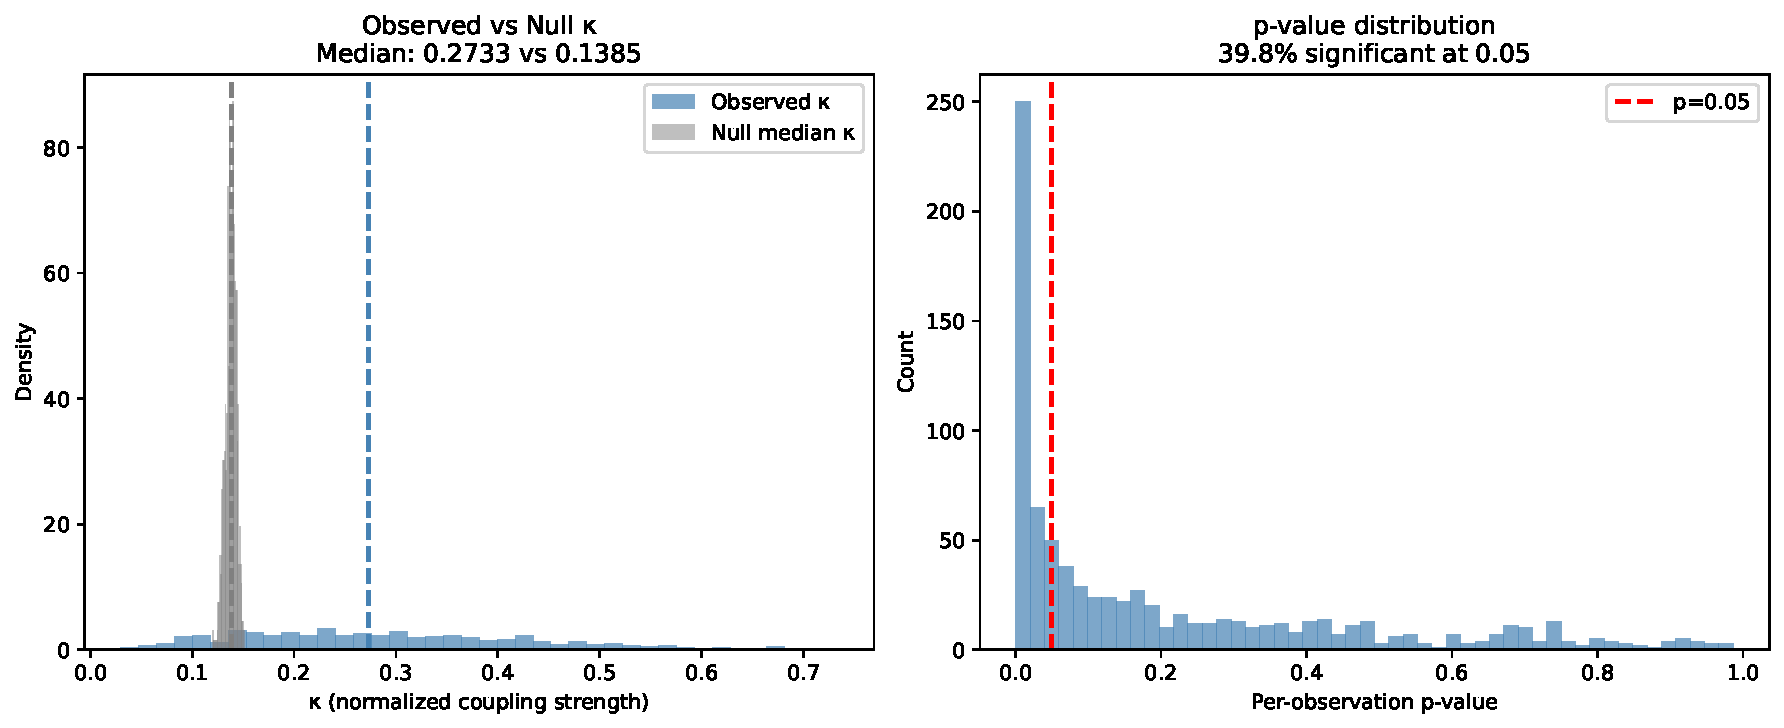
\includegraphics[width=0.95\textwidth]{pictures/chSynthesis/fig7_A2_kappa_vs_null.pdf}
\caption{Observed $\kappa$ and each observation's channel-permutation null median (left), with per-observation Monte Carlo $p$-values (right). Rows are repeated within subject and the null assumes exchangeable channel labels.}
\label{fig:kappa_null}
\end{figure}

The observed median is 0.273 (range 0.030--0.734), compared with a median of 0.139 for the per-observation null medians; 39.8\% of observations have Monte Carlo $p<0.05$ under the stated channel-permutation null. This percentage is descriptive and is not corrected across 844 tests.

\begin{figure}[htbp]
\centering
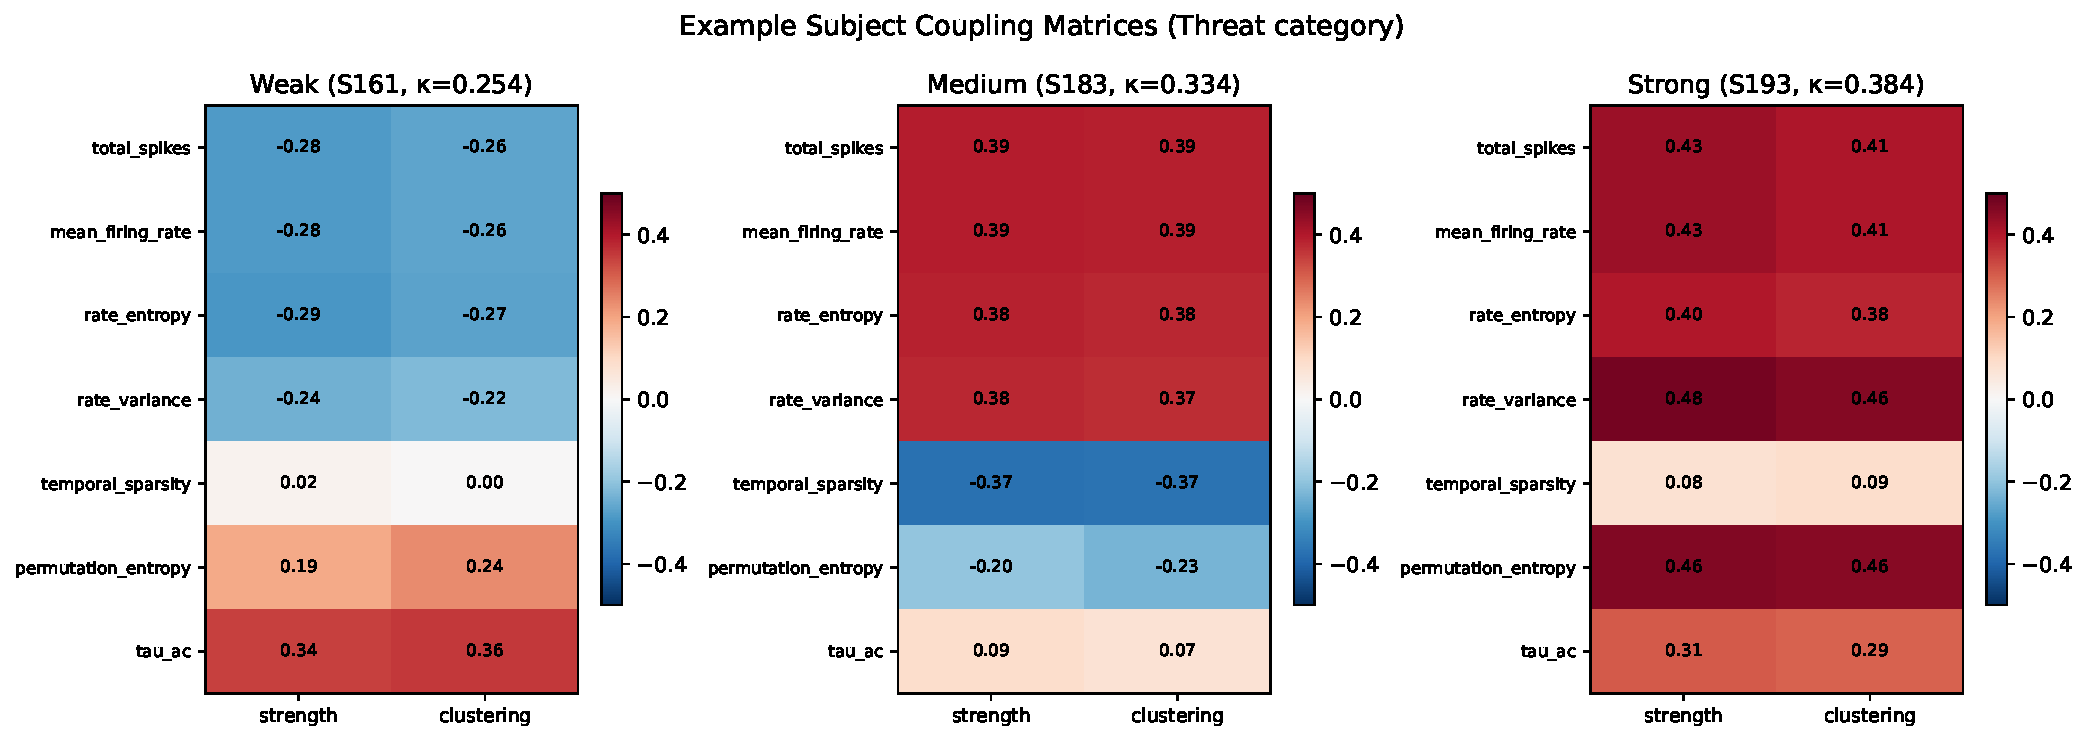
\includegraphics[width=0.95\textwidth]{pictures/chSynthesis/fig7_A3_example_subjects.pdf}
\caption{Example coupling matrices for three subjects (Threat category), selected at the 10th, 50th, and 90th percentiles of subject-mean $\kappa$. Individual-level coupling matrices show substantial inter-subject heterogeneity in both magnitude and sign pattern.}
\label{fig:example_subjects}
\end{figure}

Figure~\ref{fig:example_subjects} illustrates heterogeneity among three selected observations. Subject~161 ($\kappa = 0.254$) has negative spike-metric correlations but positive $\tau_{AC}$ correlations. Subject~183 ($\kappa = 0.334$) has the opposite pattern, and Subject~193 ($\kappa = 0.384$) has positive correlations throughout. These examples show that averaging correlations with different signs can reduce the group mean; they do not estimate the prevalence of any pattern in the population.

\subsection{Quantitative Analysis}

The archived row-level Wilcoxon test on $\kappa_{\text{obs}}-\kappa_{\text{null median}}$ gives $W=338{,}144$ and $p=4.98\times10^{-113}$; the mean difference divided by its row-level standard deviation is 1.063. Repeated rows make the $p$-value anti-conservative, and the standardized difference is not an independent-subject effect size. The descriptive shift applies only to the specified permutation null.

\begin{table}[htbp]
\centering
\caption{Coupling existence summary (Experiment~7.1).}
\label{tab:coupling_existence}
\small
\begin{tabular}{lcccc}
\toprule
\textbf{Statistic} & \textbf{Observed} & \textbf{Null median} & \textbf{$d_z$} & \textbf{$p$} \\
\midrule
Median $\kappa$ & 0.273 & 0.139 & 1.063 & $4.98 \times 10^{-113}$ \\
\% observations $p < 0.05$ & 39.8\% & 5.0\% (expected) &, &, \\
\% observations $p < 0.01$ & 23.6\% & 1.0\% (expected) &, &, \\
\bottomrule
\end{tabular}
\end{table}

The archived row-level tests flag four of 14 cells after within-matrix Bonferroni correction: permutation entropy and $\tau_{AC}$ paired with both topology summaries. The mean correlations are only $-0.044$ to $-0.051$, and the tests ignore repeated categories, so these cells are candidates for subject-level replication rather than confirmed alignments.

\subsection{Signal-Processing Interpretation}

One possible explanation is that channels with concentrated theta-band phase relationships also have more regular temporal structure, which the reservoir summaries reflect. However, tPLV, signal amplitude/spectrum, common reference, filtering, and the reservoir transform are all potential shared causes. The analysis did not measure ``input diversity'' or isolate any of these mechanisms.

The data-processing inequality does not identify the cause or direction of these correlations \cite{cover_elements_2006}; it only bounds information under deterministic transformation.

The next analysis partitions sample sums of squares in $\kappa$. This is a descriptive decomposition, not evidence that subject or category causally ``drives'' the statistic.


\section{Experiment 7.2: Variance Decomposition of Coupling Strength}
\label{sec:exp7_variance}

\subsection{Mathematical Motivation}

An archived Chapter~5 decomposition assigned 62.6\% of embedding sums of squares to subject and 8.7\% to condition, but those PCA features were fitted globally and are retained only as descriptive context. Here the balanced two-way decomposition $\kappa_{s,c}=\mu+\alpha_s+\beta_c+\varepsilon_{s,c}$ partitions sample sums of squares. It does not identify latent sources of variance or establish trait stability.

\subsection{Experimental Design}

The 844 $\kappa_{s,c}$ values are decomposed into subject, category, and residual sums of squares. Category labels are permuted within subject 5,000 times. ICC(3,1) \cite{shrout_intraclass_1979} summarizes rank consistency across four \emph{different stimulus categories}; it is not test--retest reliability because the four columns are not repeated measurements under the same condition.

\subsection{Raw Observation}

\begin{figure}[htbp]
\centering
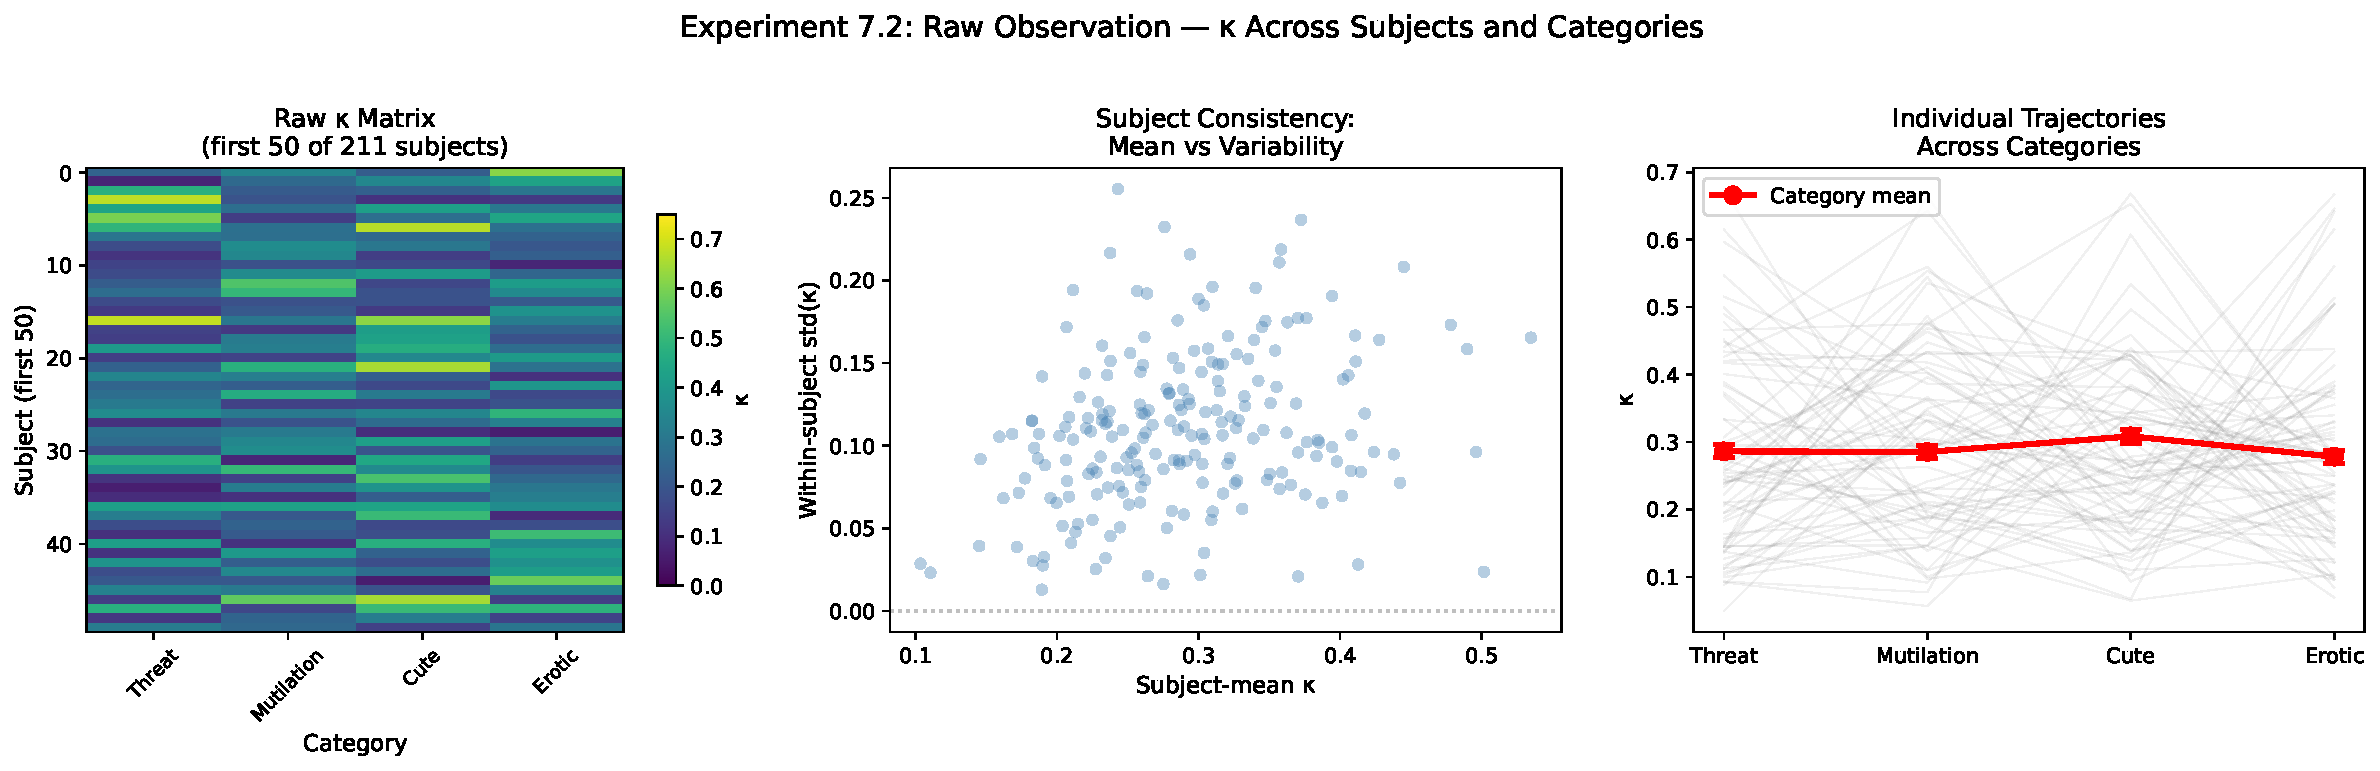
\includegraphics[width=0.95\textwidth]{pictures/chSynthesis/fig7_B1_raw_observation.pdf}
\caption{Raw observation of $\kappa$ across subjects and categories. Left: $\kappa$ matrix for the first 50 subjects (rows) $\times$ 4 categories (columns). Center: subject-mean $\kappa$ versus within-subject standard deviation. Right: individual subject trajectories across categories (gray) with category means (red). Within-subject variability (mean std $= 0.110$) exceeds between-subject variability (std of subject means $= 0.077$).}
\label{fig:raw_kappa_matrix}
\end{figure}

The category means span a narrow range: Cute ($\bar{\kappa} = 0.309$), Threat ($0.286$), Mutilation ($0.285$), Erotic ($0.278$). The between-category spread (max minus min mean) is 0.030. Within-subject standard deviation of $\kappa$ across the four categories averages 0.110, 1.43 times the between-subject standard deviation of 0.077. The individual trajectories in Figure~\ref{fig:raw_kappa_matrix} show extensive crossing: a subject with high $\kappa$ under Threat may have low $\kappa$ under Cute, and vice versa.

\begin{figure}[htbp]
\centering
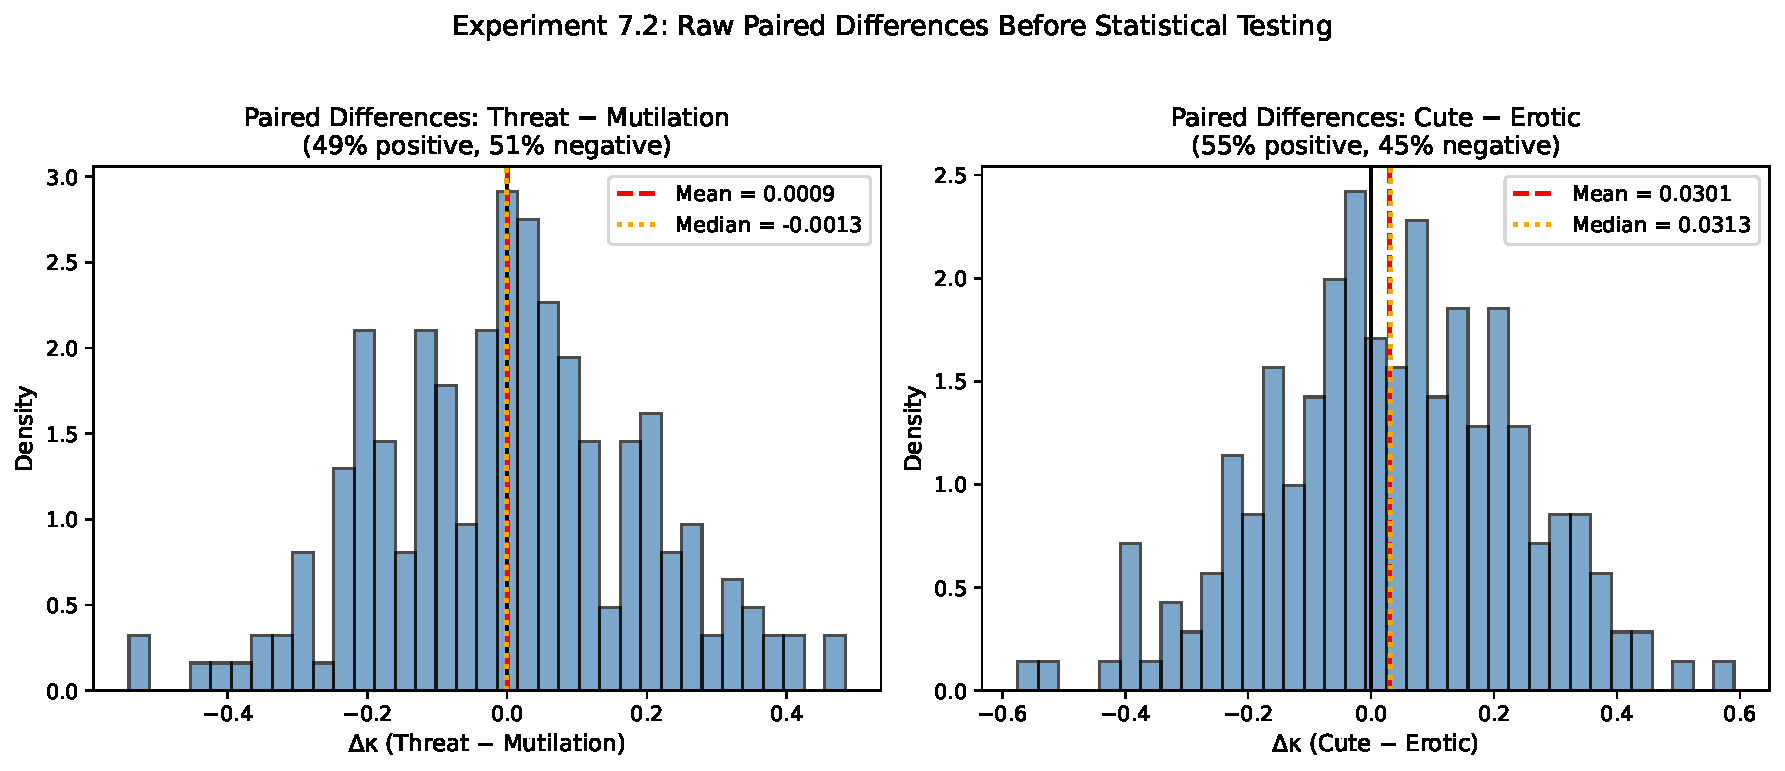
\includegraphics[width=0.95\textwidth]{pictures/chSynthesis/fig7_B2_raw_paired_differences.pdf}
\caption{Raw paired differences in $\kappa$ before statistical testing. Left: Threat $-$ Mutilation (centered on zero, 49.3\% positive). Right: Cute $-$ Erotic (shifted positive, 55.5\% positive, mean $\Delta\kappa = +0.030$).}
\label{fig:raw_paired_diff}
\end{figure}

The observed Threat--Mutilation mean difference is near zero, while the Cute--Erotic sample mean is positive. Whether that contrast exceeds the prespecified multiplicity-adjusted null is considered below.

\subsection{Quantitative Analysis}

\begin{figure}[htbp]
\centering
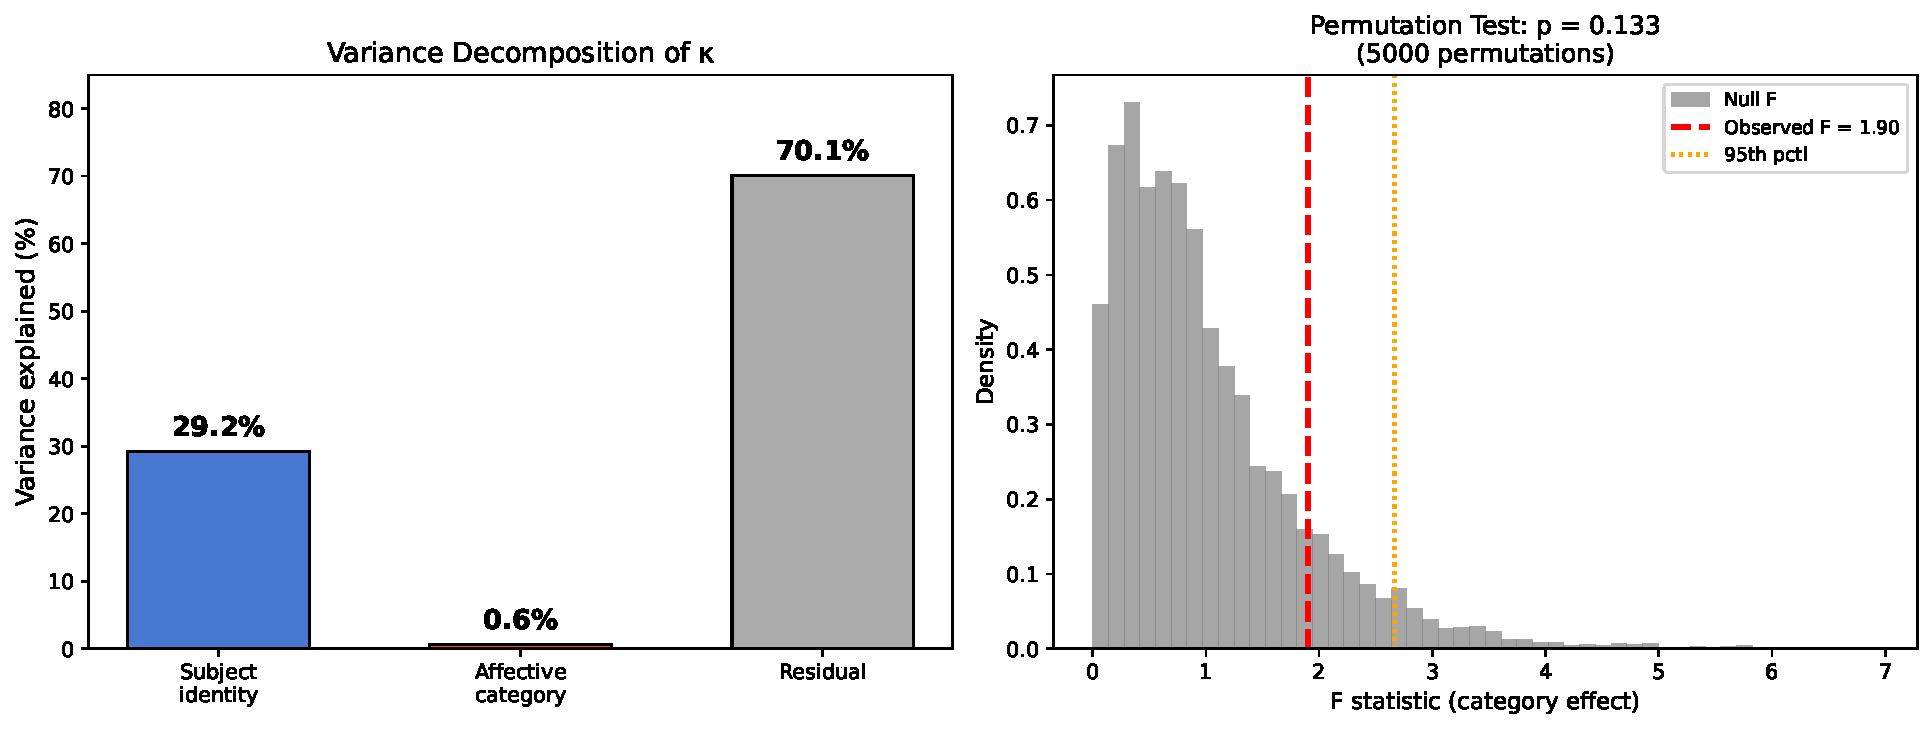
\includegraphics[width=0.95\textwidth]{pictures/chSynthesis/fig7_B3_variance_decomposition.pdf}
\caption{Left: variance decomposition of $\kappa$ into subject (29.2\%), category (0.6\%), and residual (70.1\%) components. Right: permutation null for the category $F$-statistic. The observed $F = 1.90$ falls below the 95th percentile of the null ($p = 0.133$).}
\label{fig:variance_decomp}
\end{figure}

\begin{table}[htbp]
\centering
\caption{Variance decomposition of $\kappa_{s,c}$ (Experiment~7.2).}
\label{tab:variance_decomp}
\small
\begin{tabular}{lcccc}
\toprule
\textbf{Component} & \textbf{\% Variance} & \textbf{$F$} & \textbf{$p$ (permutation)} \\
\midrule
Subject identity & 29.2\% &, &, \\
Affective category & 0.6\% & 1.90 & 0.133 \\
Residual & 70.1\% &, &, \\
\bottomrule
\end{tabular}
\end{table}

The sample sums-of-squares fractions are 29.2\% for subject, 0.6\% for category, and 70.1\% residual (Table~\ref{tab:variance_decomp}; Figure~\ref{fig:variance_decomp}). The category permutation test gives $F=1.90$, $p=0.133$, and the Friedman test gives $\chi^2=3.22$, $p=0.359$. ICC(3,1) across the four different categories is 0.059, indicating little consistency of relative ordering across those category-specific measurements; it does not prove statistical independence or poor test--retest reliability.

Threat--Mutilation gives $\Delta\kappa=-0.001$, $p=0.965$; Cute--Erotic gives $\Delta\kappa=+0.031$, $p=0.025$ without correction for the multiple planned and exploratory contrasts reported in this chapter. Because the omnibus category test is not significant, the latter is treated as a nominal exploratory result.

\subsection{Interpretation and Significance}

The subject fraction is smaller than the archived Chapter~5 fraction, but the underlying variables and preprocessing differ, so the percentages are not directly comparable. The coupling norm should not be said to ``strip away'' individual differences on this basis.

The low cross-category ICC shows that relative subject ordering changes across categories. Trait stability would require repeated sessions or repeated measurements within condition, which are unavailable.

The 70.1\% residual combines subject--category interaction, measurement error, preprocessing effects, and all unmodeled structure. It cannot be labeled genuine observation-specific neural variability without replication.

The Cute--Erotic $\kappa$ difference raises a natural question: when coupling strength increases for Cute relative to Erotic, which specific dynamical-topological relationships are driving the change?


\section{Experiment 7.3: Category-Conditioned Coupling Structure}
\label{sec:exp7_category}

\subsection{Mathematical Motivation}

The scalar $\kappa$ compresses a $7 \times 2$ matrix into one number. A Cute--Erotic difference could be spread across the 14 correlations or concentrated in a subset of cells. Chapter~\ref{chap:dynamics} grouped the descriptors into amplitude-associated summaries (total spikes, firing rate, rate entropy, rate variance) and temporal-structure summaries ($\hat{H}_\pi$, $\tau_{AC}$). The present analysis describes whether the largest sample differences occur in either group; it does not test a distinct biological pathway. The observable quantities are the 14 cell-level paired differences $\Delta\mathbf{C}_{jk} = \mathbf{C}_{\text{Cute},jk} - \mathbf{C}_{\text{Erotic},jk}$ tested with paired Wilcoxon across $N = 211$ subjects.

\subsection{Experimental Design}

For each of the two within-valence contrasts (Cute $-$ Erotic, Threat $-$ Mutilation), 14 paired Wilcoxon tests are computed across 211 subjects. Bonferroni correction within each contrast family yields $\alpha_{\text{corrected}} = 0.05/14 = 0.00357$. A secondary pattern-level test computes the Frobenius norm of the mean $\Delta\mathbf{C}$ against a sign-flip permutation null (5,000 permutations).

\subsection{Raw Observation}

\begin{figure}[htbp]
\centering
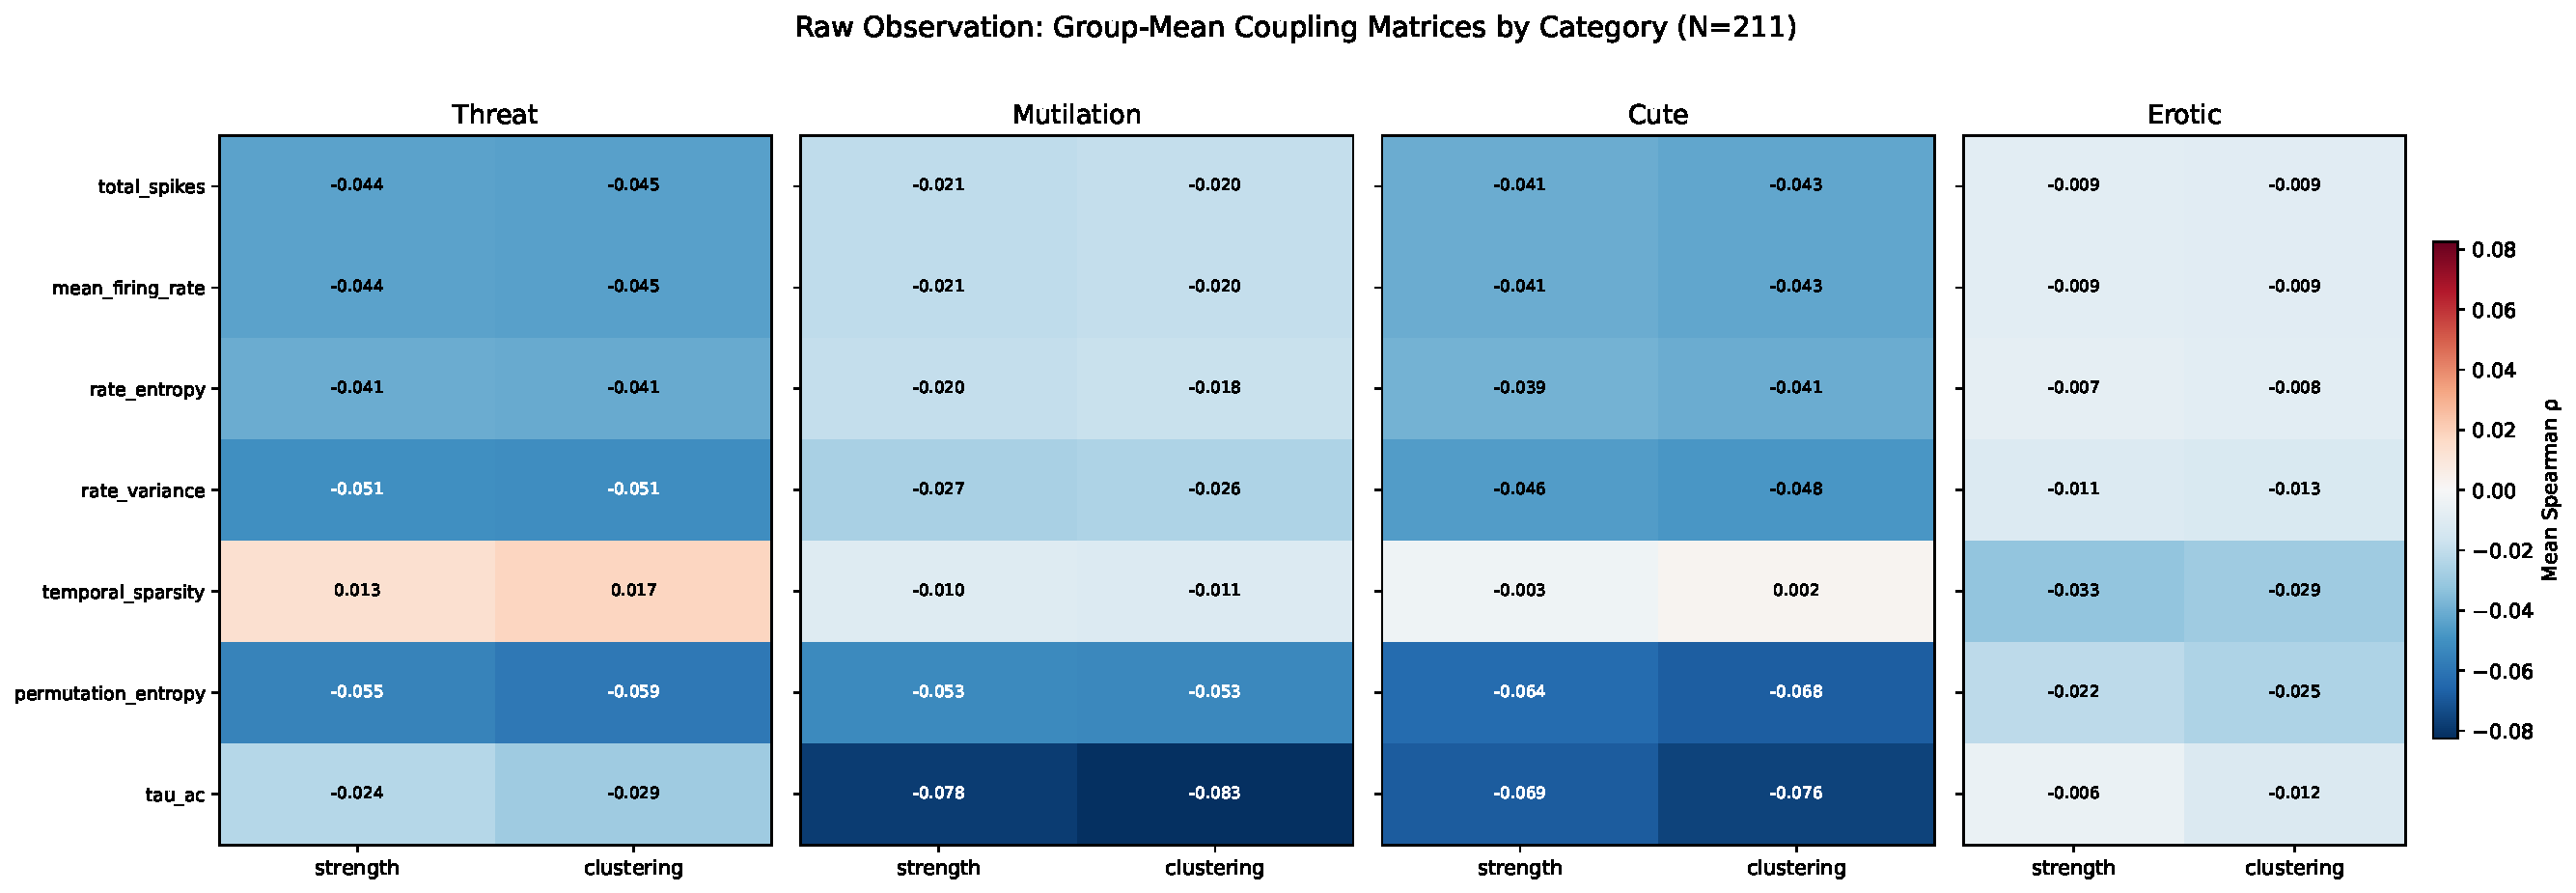
\includegraphics[width=0.95\textwidth]{pictures/chSynthesis/fig7_C1_category_C_matrices.pdf}
\caption{Group-mean coupling matrices by affective category ($N = 211$). Erotic shows the weakest coupling across all cells (most values near $-0.01$). Cute shows the strongest (permutation entropy $\times$ clustering $= -0.068$, $\tau_{AC} \times$ clustering $= -0.077$). Threat and Mutilation fall between, with different internal structures.}
\label{fig:category_C}
\end{figure}

In the sample means shown in Figure~\ref{fig:category_C}, most Erotic entries are near $-0.01$. The largest displayed Cute entries are permutation entropy $\times$ clustering at $-0.068$ and $\tau_{AC} \times$ clustering at $-0.077$. Threat and Mutilation have different sample patterns, including a Mutilation $\tau_{AC}$ correlation of $-0.083$.

\begin{figure}[htbp]
\centering
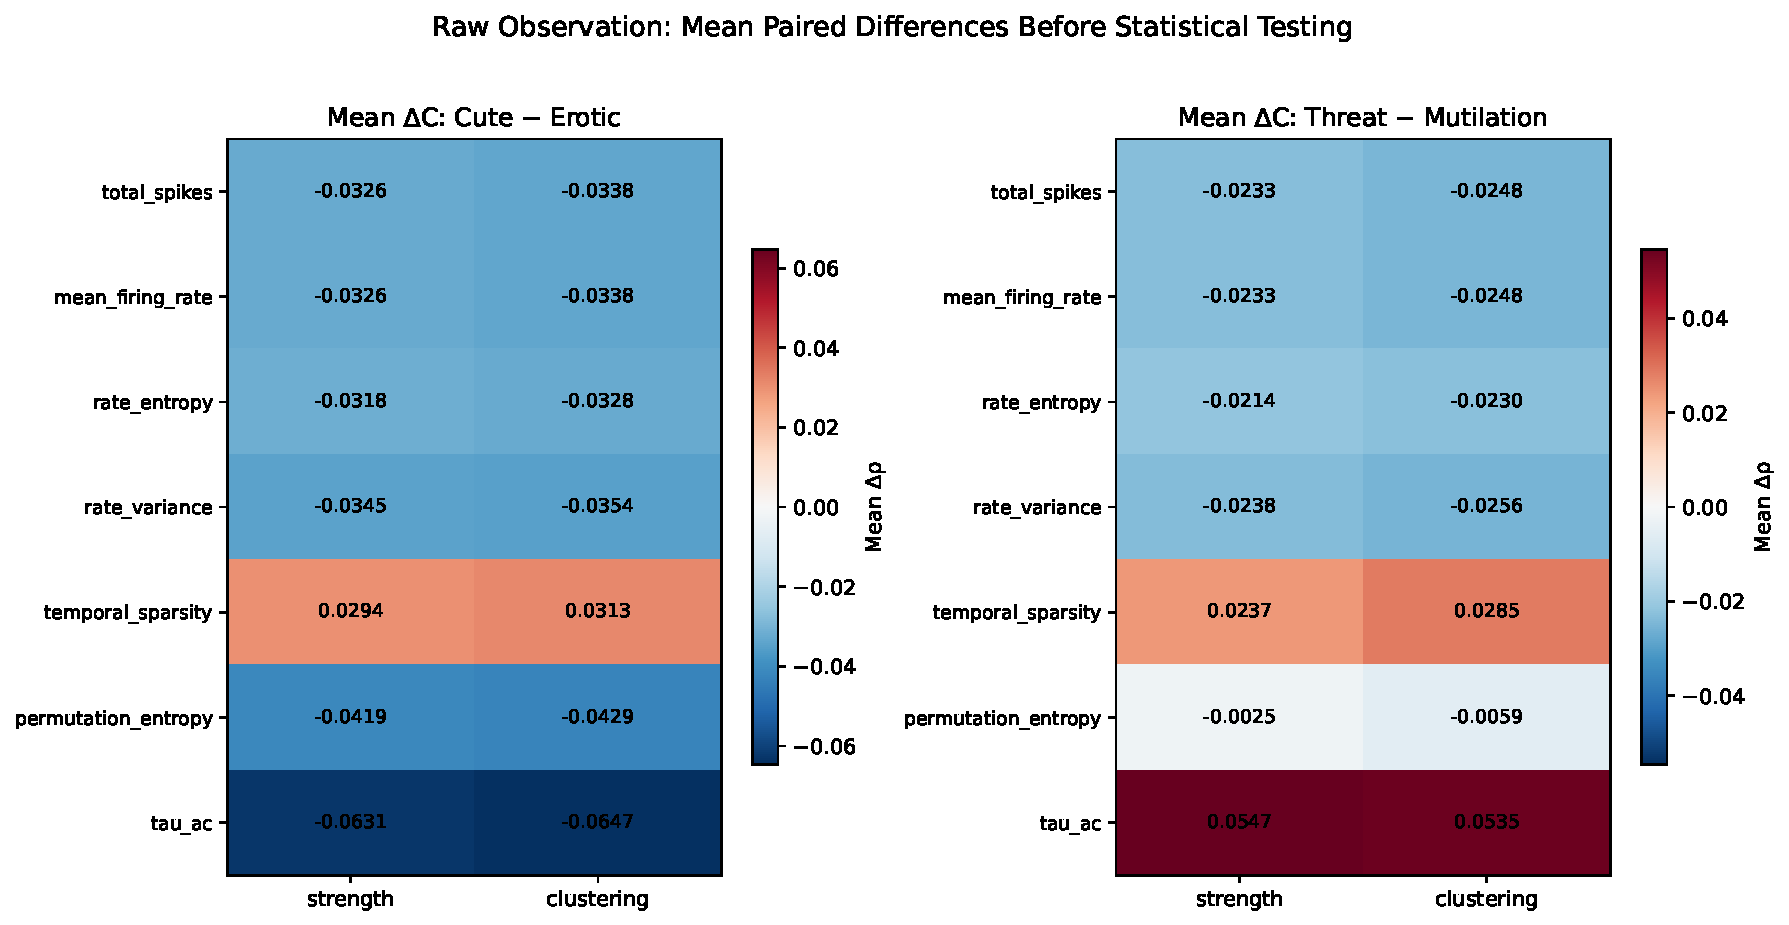
\includegraphics[width=0.95\textwidth]{pictures/chSynthesis/fig7_C2_raw_difference_matrices.pdf}
\caption{Mean paired difference matrices before statistical testing. Left: Cute $-$ Erotic shows consistent negative shifts (12 of 14 cells negative), with the largest differences in $\tau_{AC} \times$ clustering ($\Delta\rho = -0.065$) and $\tau_{AC} \times$ strength ($\Delta\rho = -0.063$). Right: Threat $-$ Mutilation shows a mixed pattern with $\tau_{AC}$ shifting in the opposite direction ($\Delta\rho = +0.054$).}
\label{fig:raw_diff_C}
\end{figure}

The raw Cute--Erotic paired differences (Figure~\ref{fig:raw_diff_C}) are negative in 12 of 14 cells, with only 43.1--46.9\% of subjects showing positive $\Delta\rho$ on the largest cells. The $\tau_{AC}$ row carries the largest shifts: $\Delta\rho = -0.065$ for $\tau_{AC} \times$ clustering and $-0.063$ for $\tau_{AC} \times$ strength.

\subsection{Quantitative Analysis}

\begin{figure}[htbp]
\centering
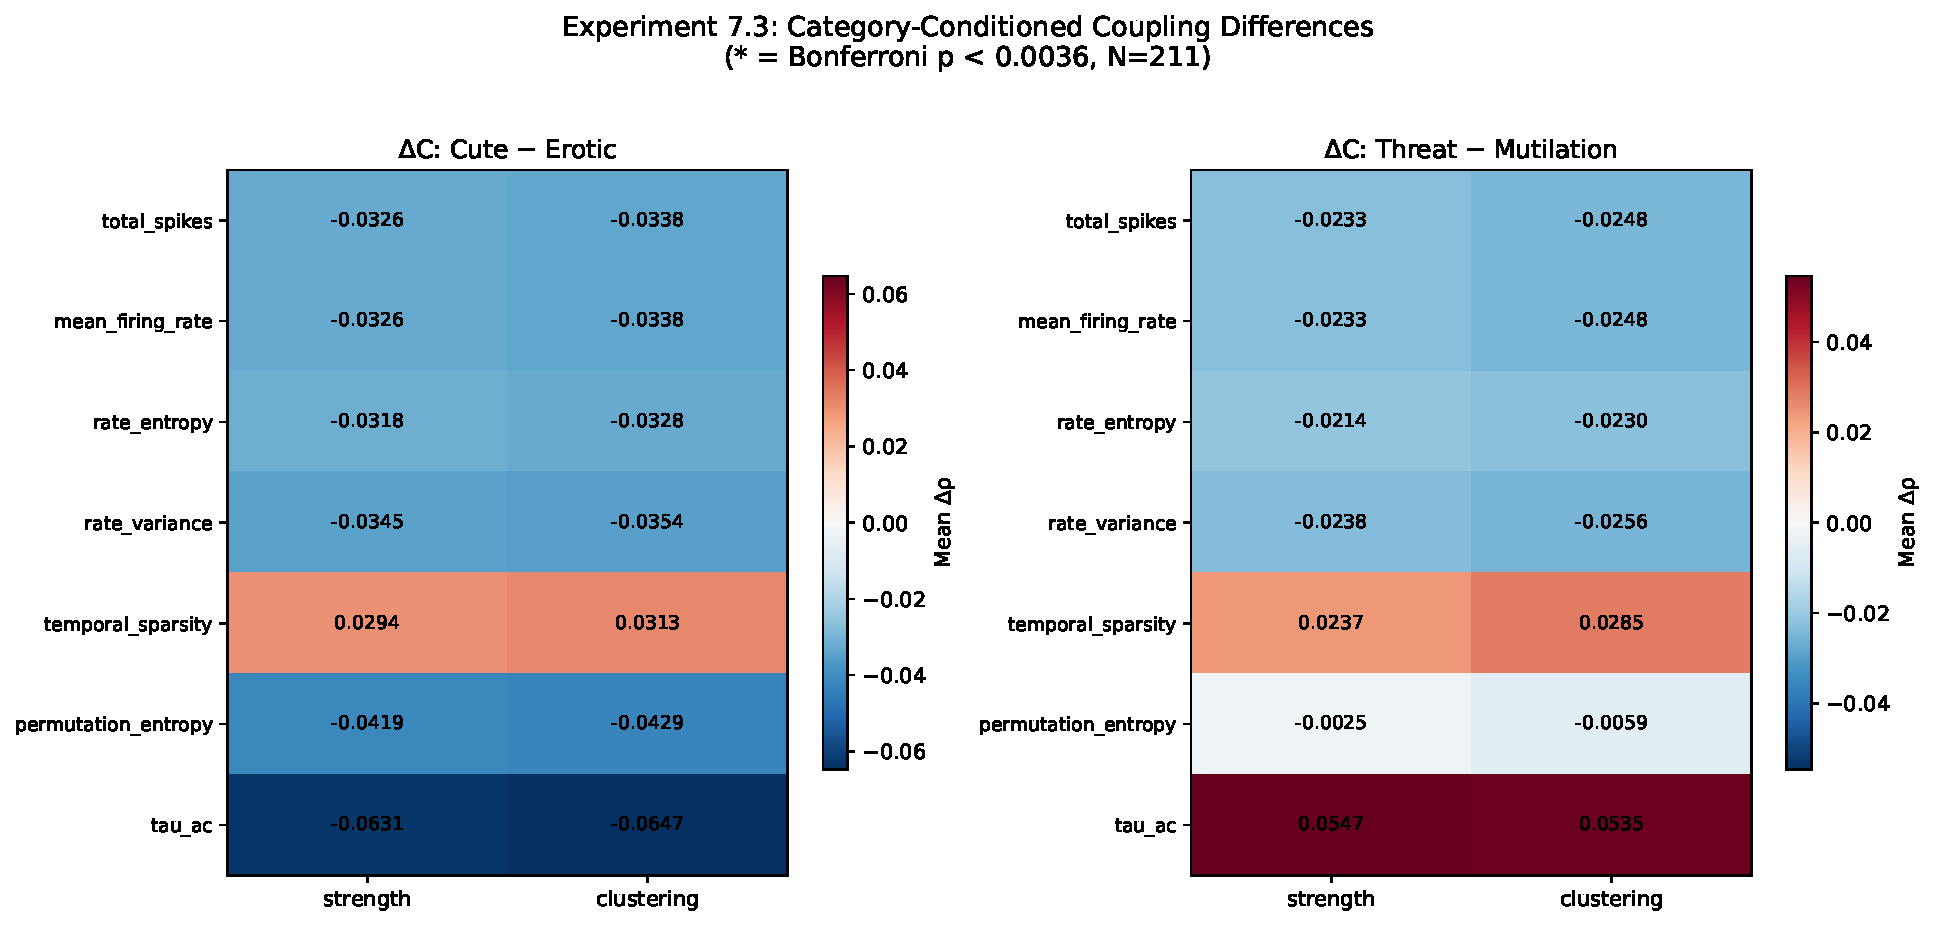
\includegraphics[width=0.95\textwidth]{pictures/chSynthesis/fig7_C3_difference_significance.pdf}
\caption{Difference matrices with Bonferroni significance masking ($\alpha = 0.05/14$). No individual cell reaches Bonferroni significance for either contrast. The $\tau_{AC}$ cells for Cute $-$ Erotic reach $p = 0.013$--$0.016$ uncorrected.}
\label{fig:diff_significance}
\end{figure}

No individual cell reaches Bonferroni significance for either within-valence contrast (0 of 14 for both; Figure~\ref{fig:diff_significance}). The closest are $\tau_{AC} \times$ clustering ($p = 0.013$, $d_z = 0.161$) and $\tau_{AC} \times$ strength ($p = 0.016$, $d_z = 0.155$) for Cute $-$ Erotic. The pattern-level Frobenius test is also non-significant (Cute $-$ Erotic: $\|\Delta\mathbf{C}\|_F = 0.150$, $p = 0.177$; Threat $-$ Mutilation: $\|\Delta\mathbf{C}\|_F = 0.109$, $p = 0.277$).

The temporal-structure group has the larger descriptive Cute--Erotic effect-size average (mean $|d_z| = 0.129$, minimum uncorrected $p = 0.013$), about $1.8\times$ the amplitude-associated group (mean $|d_z| = 0.072$, minimum uncorrected $p = 0.237$). This ratio was computed after grouping and inspecting the results and is not a confirmatory interaction test.

\subsection{Interpretation and Significance}

The Cute--Erotic sample difference is spread across 12 of 14 mean cells. However, no cell survives correction and the pattern-level Frobenius test is non-significant ($p=0.177$). The data therefore do not establish coordinated pattern-level modulation.

The largest uncorrected shifts occur for the two temporal-structure summaries. This is a hypothesis-generating rank ordering, not evidence of a distinct pathway or cross-chapter mechanism.

For Threat--Mutilation, the largest $\tau_{AC}$ comparison has $\Delta\rho=+0.054$ and uncorrected $p=0.024$. It does not survive the stated family correction and cannot establish content-specific reorganization.

A prospective replication should base sample size on an independently specified effect and analysis plan; a post-hoc calculation from the current selected cells is optimistic. The next section examines diagnosis-associated differences exploratorily.


\section{Experiment 7.4: Diagnosis-Group Comparisons}
\label{sec:exp7_diagnosis}

\subsection{Mathematical Motivation}

Earlier exploratory analyses reported diagnosis-associated descriptor differences. This section asks whether subject-mean coupling differs between one-versus-rest groups. The observable is $\Delta\bar{\kappa}=\bar{\kappa}_{\mathrm{Dx}^+}-\bar{\kappa}_{\mathrm{Dx}^-}$, where $\bar{\kappa}_s=\frac14\sum_c\kappa_{s,c}$.

All diagnosis comparisons are one-versus-rest within a transdiagnostic sample. The mean count is 2.0 among the five primary labels tested here; the broader supplied panel has mean 2.8. Results are diagnosis-associated coupling differences conditioned by that comorbidity structure, not disorder-specific signatures.

\subsection{Experimental Design}

Five diagnoses are tested: MDD ($n^+ = 142$, $n^- = 64$), SUD ($n^+ = 85$, $n^- = 121$), PTSD ($n^+ = 82$, $n^- = 124$), GAD ($n^+ = 60$, $n^- = 146$), and ADHD ($n^+ = 50$, $n^- = 156$). Group comparisons use Mann--Whitney~$U$ on $\bar{\kappa}_s$ with Bonferroni correction across five tests ($\alpha = 0.01$). A secondary analysis tests diagnosis $\times$ category interactions by permutation (5,000 iterations). Power analysis reports the minimum detectable Cohen's~$d$ at $\alpha = 0.05$, power $= 0.80$ for each comparison.

\subsection{Raw Observation}

\begin{figure}[htbp]
\centering
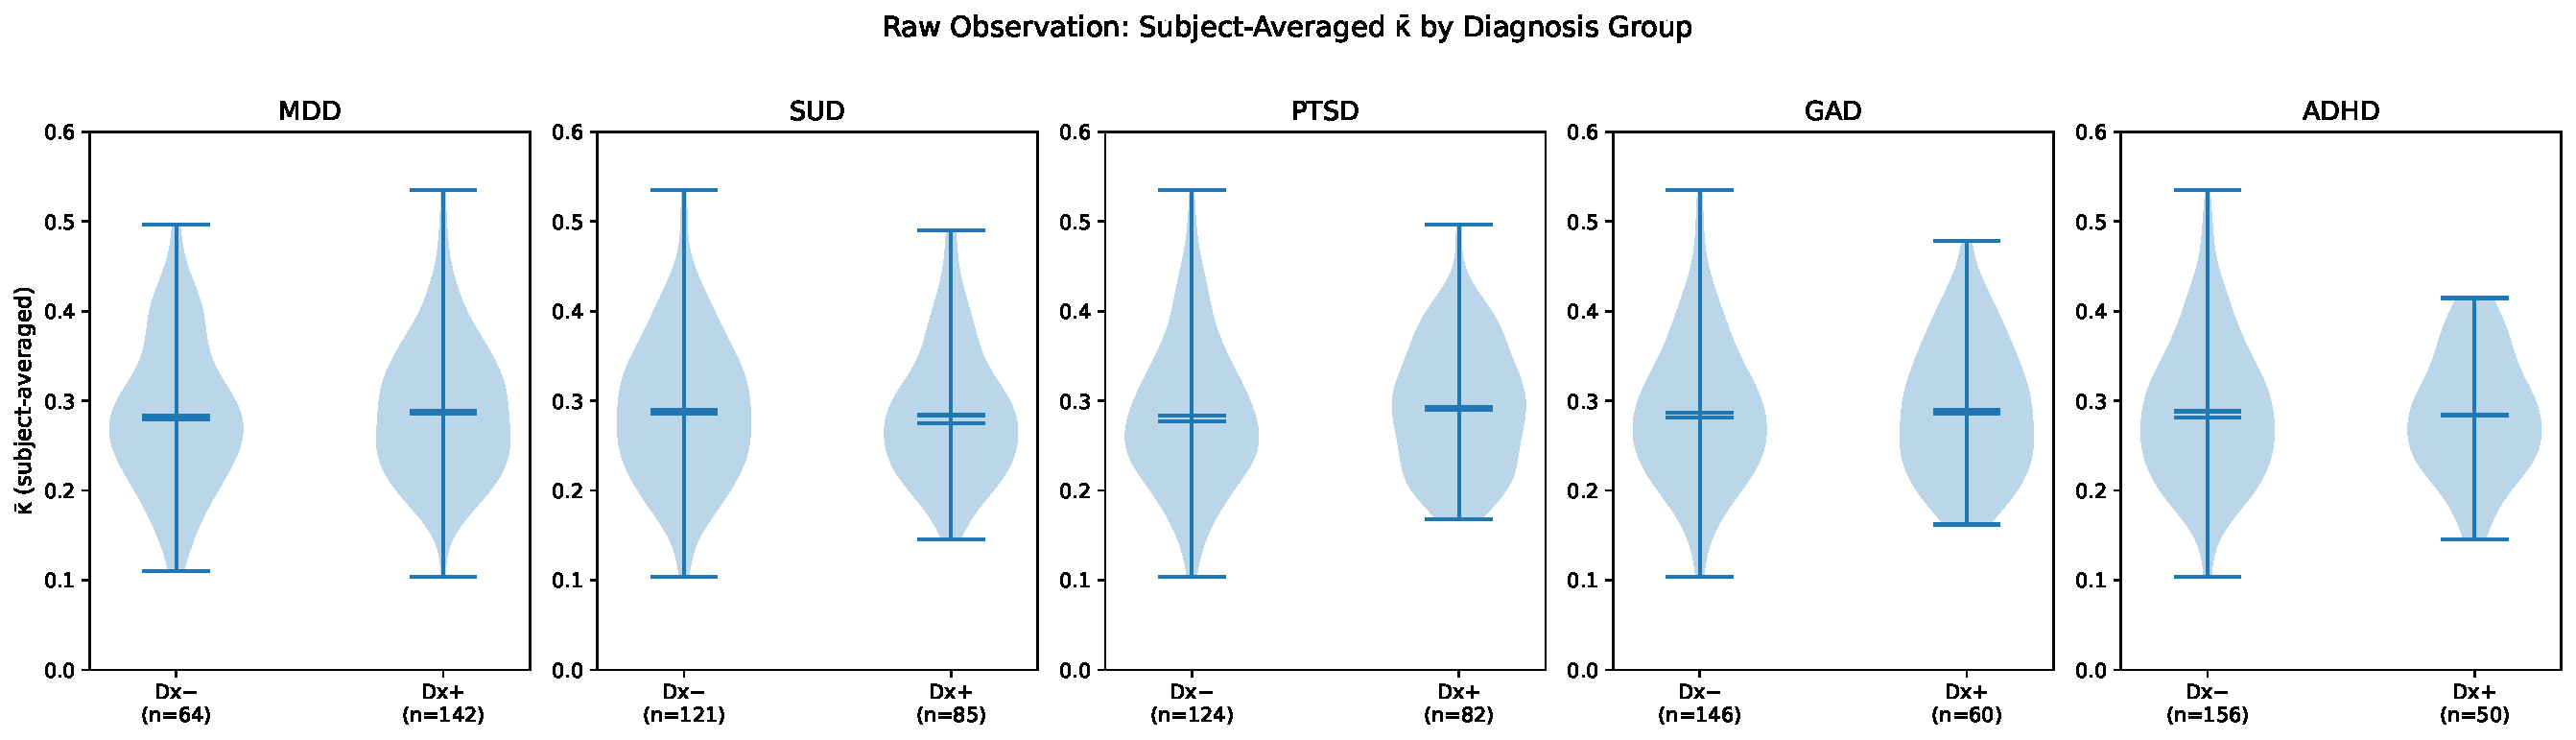
\includegraphics[width=0.95\textwidth]{pictures/chSynthesis/fig7_D1_raw_diagnosis_kappa.pdf}
\caption{Subject-averaged $\bar{\kappa}$ by diagnosis group for five diagnoses. The Dx$^+$ and Dx$^-$ distributions overlap extensively for all diagnoses. No visible separation is present in the raw violin plots.}
\label{fig:raw_diag_kappa}
\end{figure}

The raw violin plots (Figure~\ref{fig:raw_diag_kappa}) show near-complete distributional overlap between Dx$^+$ and Dx$^-$ for all five diagnoses. Group means differ by at most 0.009 (PTSD: $\bar{\kappa}_{\text{Dx}^+} = 0.293$ versus $\bar{\kappa}_{\text{Dx}^-} = 0.284$). The within-group standard deviations ($\approx 0.07$) are an order of magnitude larger than the between-group mean differences.

\subsection{Quantitative Analysis}

\begin{table}[htbp]
\centering
\caption{Diagnosis-associated coupling differences (Experiment~7.4).}
\label{tab:diagnosis_coupling}
\small
\begin{tabular}{lccccccc}
\toprule
\textbf{Dx} & \textbf{$n^+$} & \textbf{$n^-$} & \textbf{$\bar{\kappa}^+$} & \textbf{$\bar{\kappa}^-$} & \textbf{$d$} & \textbf{$p$} & \textbf{MDE} \\
\midrule
MDD & 142 & 64 & 0.289 & 0.283 & $+0.081$ & 0.609 & 0.42 \\
SUD & 85 & 121 & 0.284 & 0.290 & $-0.075$ & 0.485 & 0.40 \\
PTSD & 82 & 124 & 0.293 & 0.284 & $+0.116$ & 0.322 & 0.40 \\
GAD & 60 & 146 & 0.290 & 0.287 & $+0.043$ & 0.762 & 0.43 \\
ADHD & 50 & 156 & 0.285 & 0.288 & $-0.051$ & 0.921 & 0.46 \\
\bottomrule
\end{tabular}
\end{table}

No comparison reaches the five-test corrected threshold (Table~\ref{tab:diagnosis_coupling}); sample Cohen's~$d$ values are below 0.12. The reported minimum detectable effects of about 0.40--0.46 show that the study was not designed to exclude small differences. The result is therefore lack of evidence for a moderate or large scalar difference, not proof of absence.

\begin{figure}[htbp]
\centering
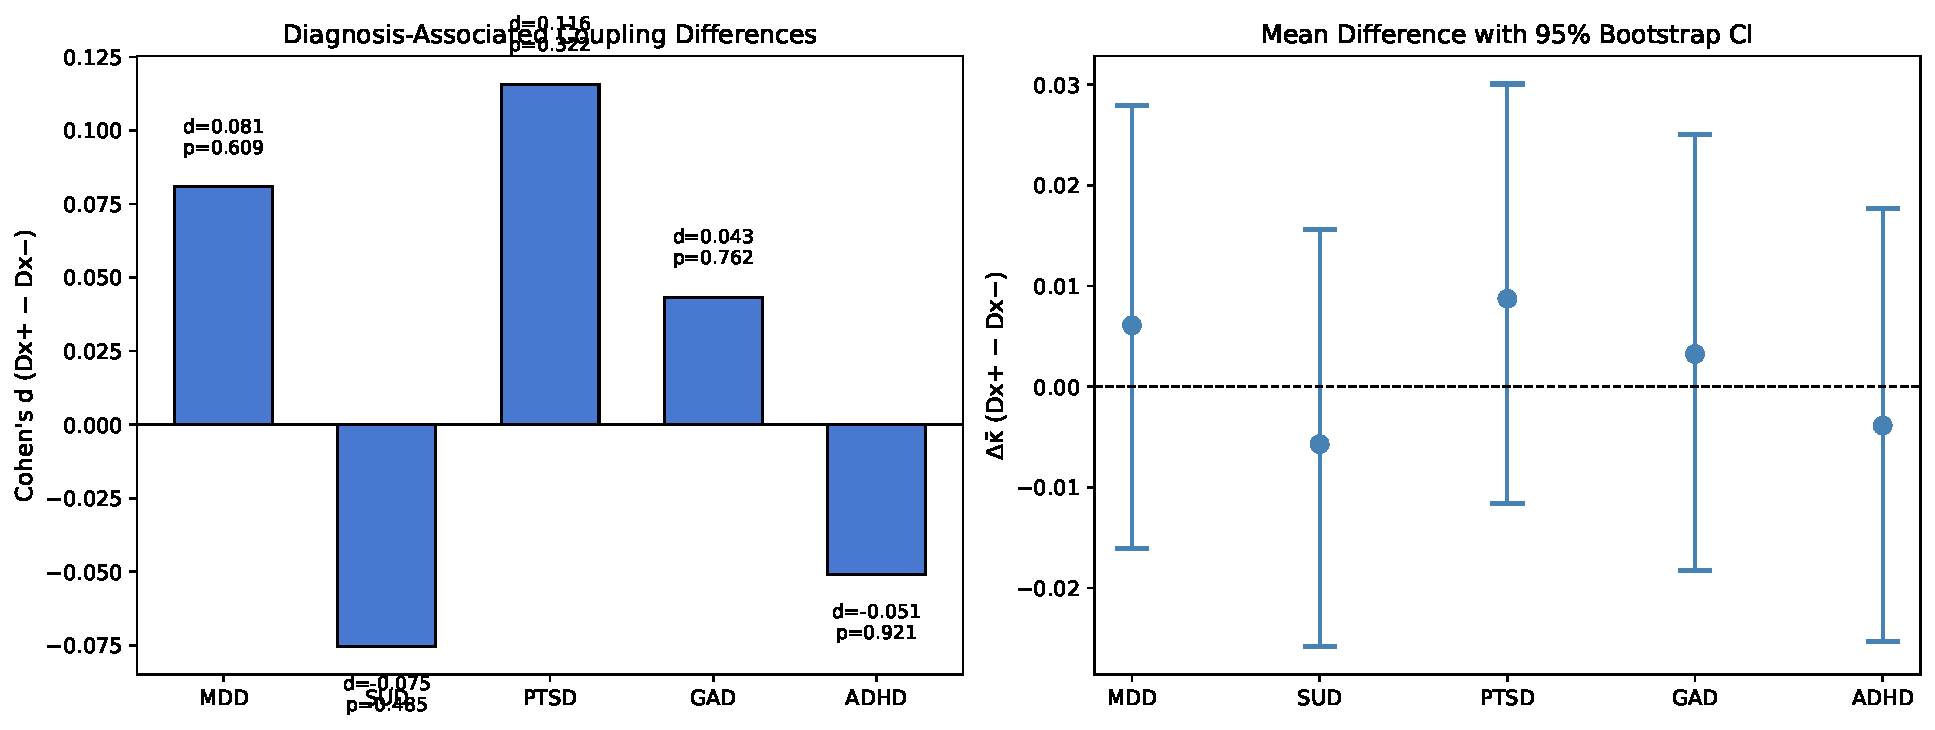
\includegraphics[width=0.95\textwidth]{pictures/chSynthesis/fig7_D2_diagnosis_effects.pdf}
\caption{Left: Cohen's~$d$ for each diagnosis. All values are below $|d| = 0.12$. Right: bootstrap 95\% confidence intervals for the mean $\bar{\kappa}$ difference. All intervals include zero.}
\label{fig:diagnosis_effects}
\end{figure}

The secondary diagnosis $\times$ category interaction analysis identifies one suggestive pattern: ADHD shows a category-dependent coupling profile with the lowest $\kappa$ for Mutilation (0.261) and the highest for Erotic (0.308), reaching $p = 0.035$ uncorrected. This does not survive Bonferroni correction across five diagnoses and is carried forward as a hypothesis for future investigation.

\subsection{Interpretation and Significance}

Within this one-versus-rest, comorbid sample, subject-mean $\kappa$ does not show corrected diagnosis-group separation. This does not demonstrate equivalence, and it should not be used to infer that the individual descriptor families contain disorder-specific effects.

The ADHD interaction has uncorrected $p=0.035$ and does not survive the five-diagnosis correction. It is retained only as a hypothesis.

A natural question follows: if coupling is organizationally informative but not diagnosis-discriminative at the scalar level, do the individual descriptor families carry complementary discriminative information when combined?


\section{Experiment 7.5: Augmentation Ablation}
\label{sec:exp7_augmentation}

\subsection{Mathematical Motivation}

The final four-category analysis compares linear-readout AUC for topology, dynamics, their concatenation, and concatenation plus $\kappa$. It is an exploratory model comparison, not a test of clinical detection utility.

\subsection{Experimental Design}

Four feature conditions are constructed from subject-averaged per-electrode descriptors: T-only (68 features: 34 electrodes $\times$ 2 topology metrics), D-only (238 features: 34 electrodes $\times$ 7 dynamical metrics), T+D (306 features: concatenation), and T+D+$\kappa$ (307 features: concatenation plus subject-averaged coupling strength). Five binary detection tasks are tested: SUD, MDD, PTSD, GAD, and ADHD. The primary readout is $L_2$-regularized logistic regression ($C = 1.0$) with subject-level stratified 5-fold cross-validation repeated 10 times (50 total folds).

\subsection{Raw Observation}

\begin{figure}[htbp]
\centering
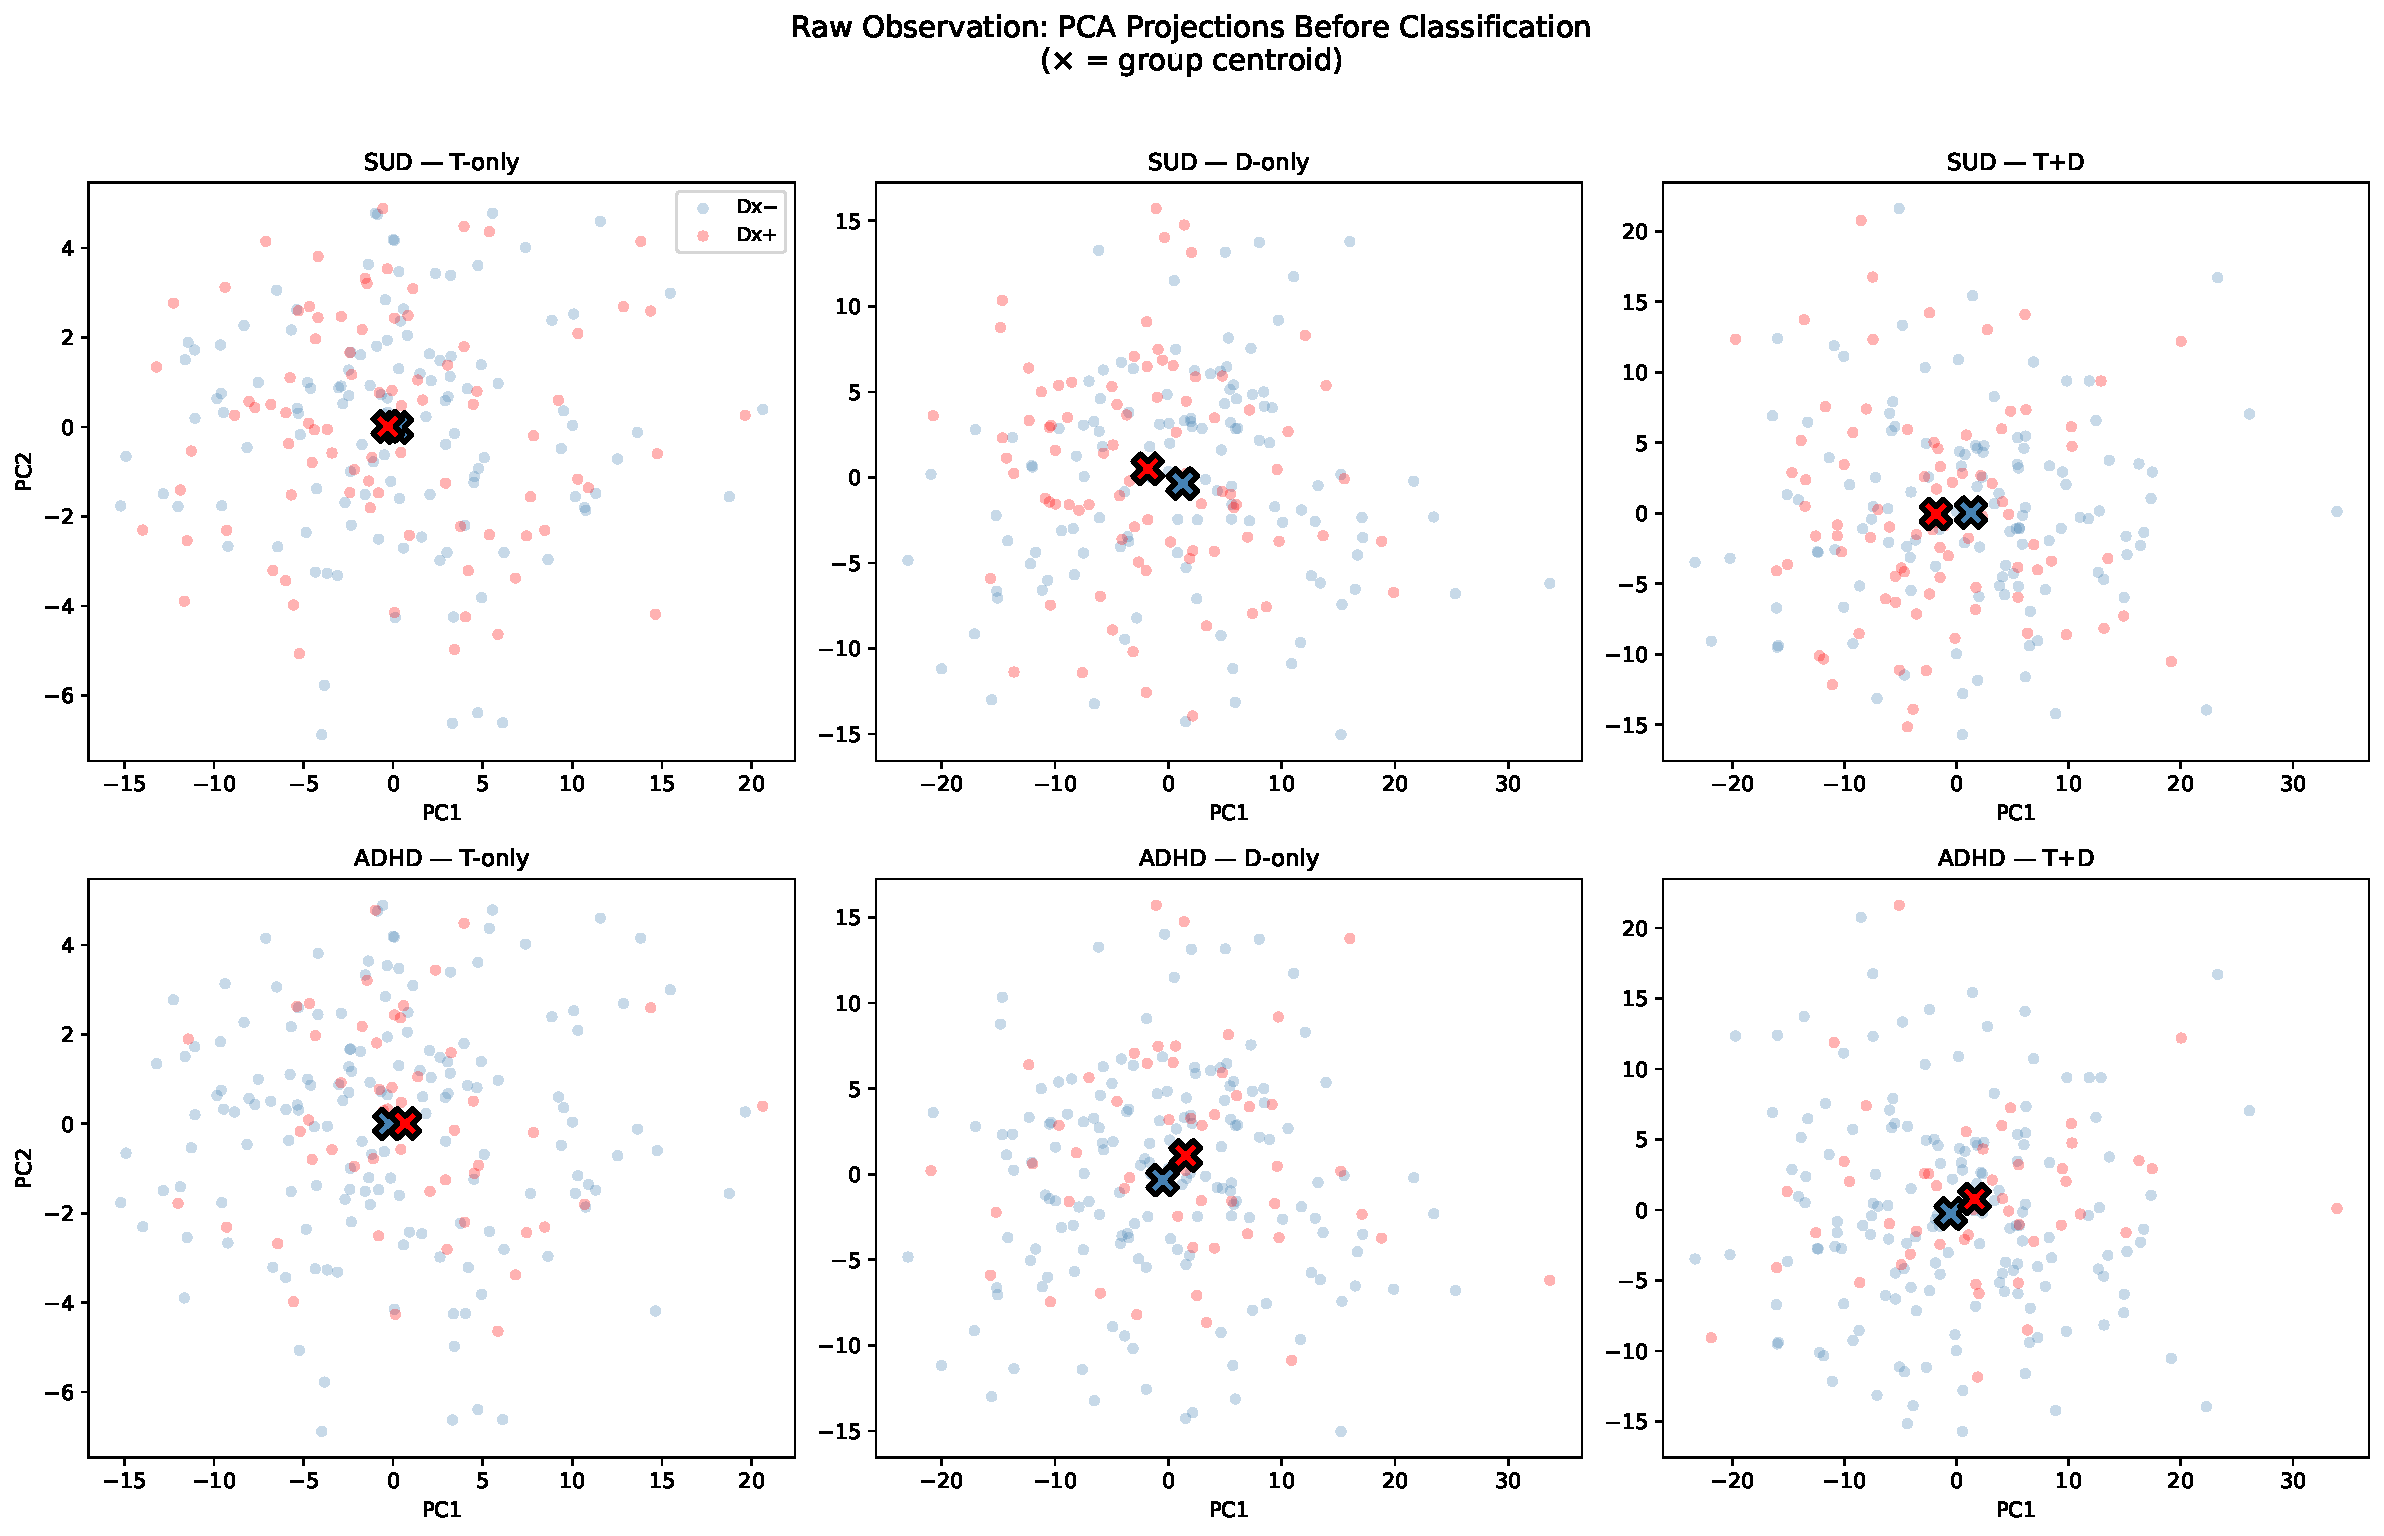
\includegraphics[width=0.95\textwidth]{pictures/chSynthesis/fig7_E1_raw_pca_projections.pdf}
\caption{PCA projections before classification for SUD (top) and ADHD (bottom) across T-only, D-only, and T+D feature spaces. Group centroids ($\times$) are marked. SUD shows near-complete overlap in all three spaces. ADHD shows visible D-only centroid offset that is absent in T-only.}
\label{fig:pca_projections}
\end{figure}

The dynamics and concatenated matrices have more columns than independent subjects and are rank-deficient. Full-sample PCA plots are visualization only and cannot predict held-out performance. The counts of univariate $p<0.05$ are uncorrected screens across hundreds of features and are not evidence of localized effects.

\begin{figure}[htbp]
\centering
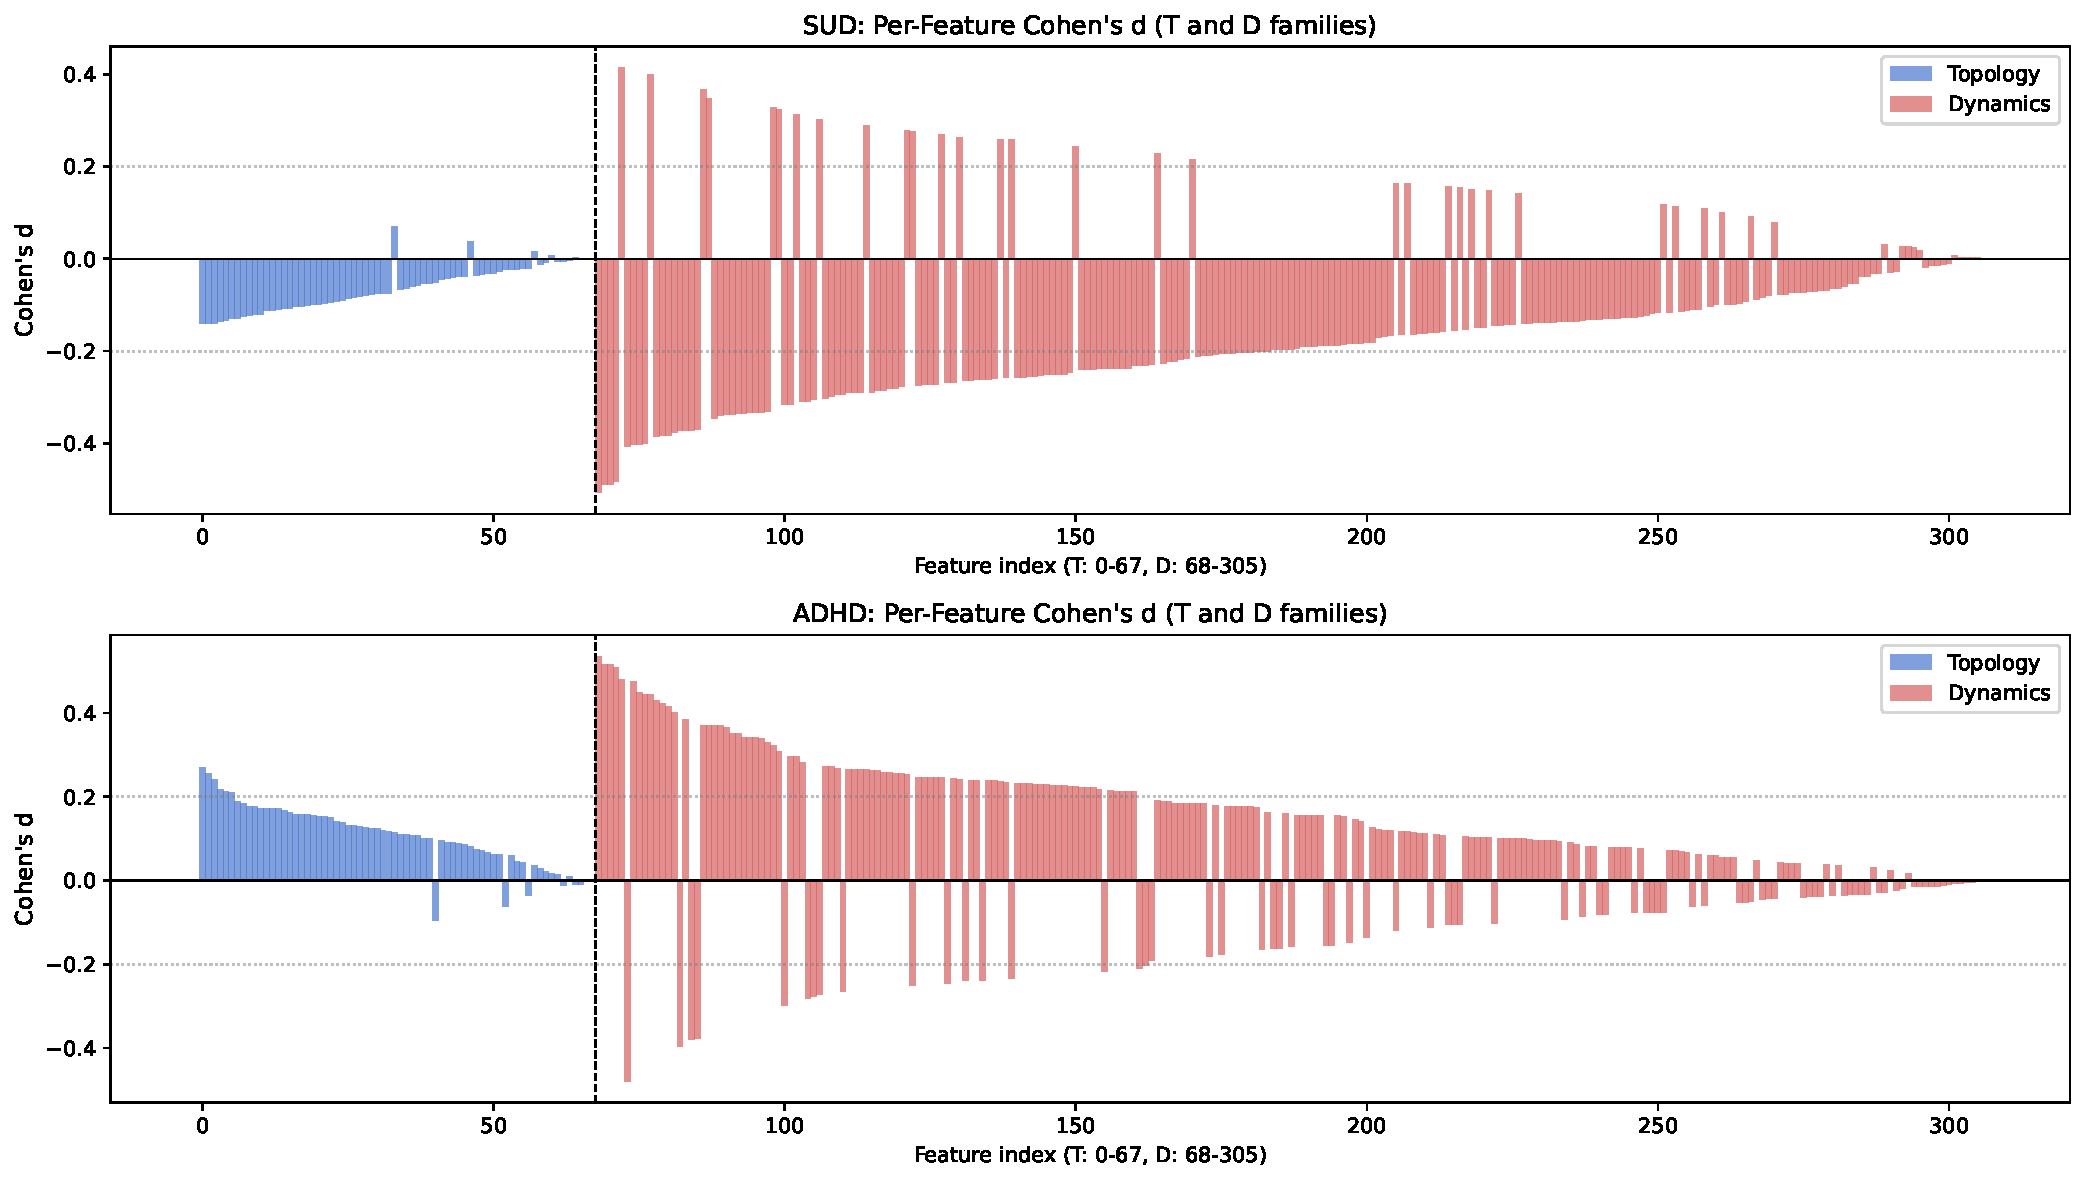
\includegraphics[width=0.95\textwidth]{pictures/chSynthesis/fig7_E2_raw_univariate_effects.pdf}
\caption{Per-feature Cohen's~$d$ across all 306 features for SUD (top) and ADHD (bottom). Topology features (left of vertical line) cluster near $d = 0$. Dynamics features (right) show scattered effects, broader for ADHD than SUD.}
\label{fig:univariate_effects}
\end{figure}

These plots motivated, but did not preregister or guarantee, the subsequent classifier comparison.

\subsection{Quantitative Analysis}

\begin{table}[htbp]
\centering
\caption{Augmentation comparison: mean AUC and standard deviation across 50 overlapping repeated-CV folds. Fold standard deviations are not confidence intervals.}
\label{tab:augmentation}
\small
\begin{tabular}{lcccc}
\toprule
\textbf{Dx} & \textbf{T-only} & \textbf{D-only} & \textbf{T+D} & \textbf{T+D+$\kappa$} \\
\midrule
SUD & $0.464 \pm 0.071$ & $0.464 \pm 0.076$ & $0.458 \pm 0.083$ & $0.455 \pm 0.082$ \\
MDD & $0.518 \pm 0.094$ & $0.504 \pm 0.085$ & $0.512 \pm 0.092$ & $0.510 \pm 0.090$ \\
PTSD & $0.487 \pm 0.072$ & $0.527 \pm 0.073$ & $0.510 \pm 0.069$ & $0.505 \pm 0.069$ \\
GAD & $\mathbf{0.581} \pm 0.092$ & $0.533 \pm 0.093$ & $0.568 \pm 0.084$ & $0.563 \pm 0.083$ \\
ADHD & $0.533 \pm 0.077$ & $\mathbf{0.622} \pm 0.086$ & $0.597 \pm 0.076$ & $0.608 \pm 0.084$ \\
\bottomrule
\end{tabular}
\end{table}

In the recorded repeated splits, SUD AUC is about 0.46 across conditions; the largest mean is 0.622 for ADHD with dynamics, and the largest GAD mean is 0.581 with topology. Concatenation does not exceed the better single family for any of the five labels in this finite comparison.

\begin{figure}[htbp]
\centering
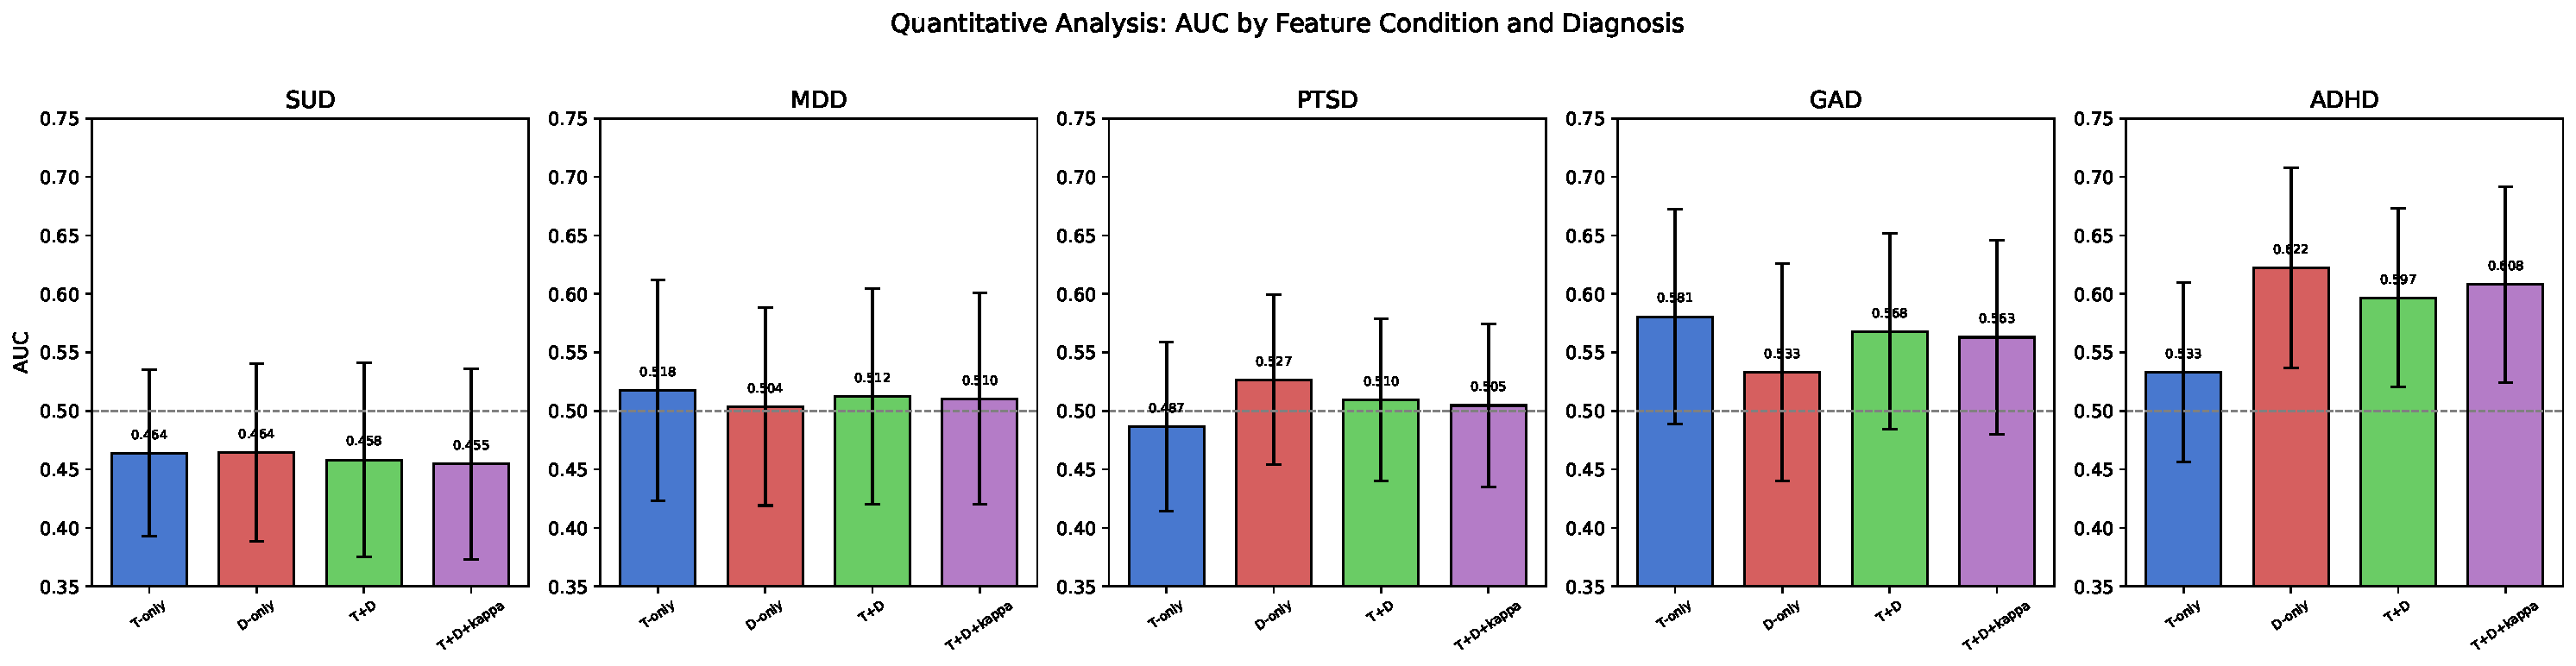
\includegraphics[width=0.95\textwidth]{pictures/chSynthesis/fig7_E4_classification_auc.pdf}
\caption{Mean repeated-CV AUC by feature condition and diagnosis. Bold values mark the largest sample mean per diagnosis; they are not multiplicity-adjusted claims of above-chance clinical performance.}
\label{fig:classification_auc}
\end{figure}

For ADHD, the recorded mean changes from 0.622 (D-only) to 0.597 (T+D) and 0.608 (T+D+$\kappa$). The archived $p$-values treated 50 overlapping fold scores as independent and are invalid; they are not used. These small mean differences do not establish non-redundant ADHD information.

\subsection{Interpretation and Significance}

The narrow conclusion is that concatenation did not improve the sample mean AUC in these models and splits. That does not prove the feature families lack complementary information under other estimators or cohorts.

The per-diagnosis maxima are post-hoc model-selection observations. They do not show diagnosis specificity or support a complete clinical characterization.

The ADHD interaction and augmentation observations arise from the same cohort and are not independent replications. One is uncorrected and the other relied on invalid fold-level inference. They are retained only as exploratory prompts for a prespecified external study.


\section{Separate Three-Condition Analysis}
\label{sec:ch7_3class}

This section reports a separate Negative/Neutral/Pleasant pipeline. It is not a replication of the four-category analysis because the observations, preprocessing, and archived reservoir update differ. Archived PCA-based condition-variance ratios are also affected by global PCA fitting and do not imply tighter confidence intervals. The comparison below is therefore a cross-pipeline sensitivity analysis.

\subsection{Coupling Existence at Three-Class}

The mean coupling scalar is $\kappa=0.221\pm0.111$. None of 5,000 permuted means equaled or exceeded the observed mean. With the standard plus-one Monte Carlo correction, the result is $p=1/5001\approx0.0002$, not zero. The corrected script uses this calculation; the archived figure's displayed zero was generated before the audit.

Six of the 14 sample-mean entries are negative and eight positive. Their signs and magnitudes describe cross-channel association in this pipeline; they do not show that connectivity produces a particular reservoir response. The contrast with the four-category sign pattern is confounded by the different archived implementations.

\begin{figure}[H]
    \centering
    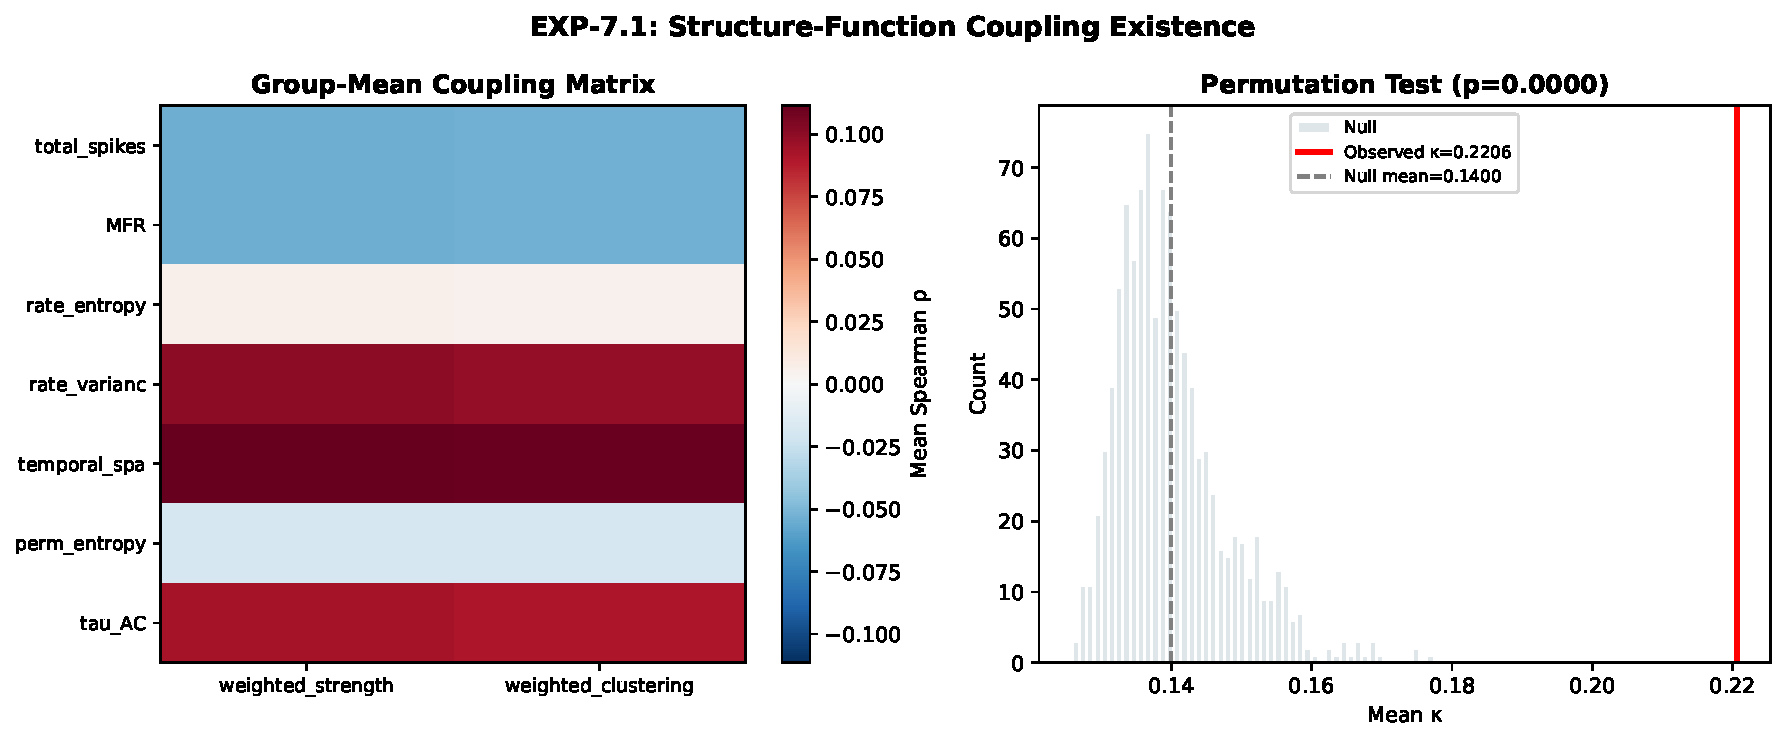
\includegraphics[width=\textwidth]{pictures/chSynthesis/fig_3class_coupling_existence.pdf}
    \caption{Three-condition coupling summary ($N=211$, 633 observations). The mean matrix has six negative and eight positive entries. The archived plot labels the 5,000-permutation result as zero; the corrected plus-one Monte Carlo value is $p=1/5001\approx0.0002$.}
    \label{fig:ch7_3class_coupling}
\end{figure}

\subsection{Variance Decomposition at Three-Class}

The sample sums-of-squares fractions are 40.3\% subject, 0.7\% condition, and 59.0\% residual (Figure~\ref{fig:ch7_3class_variance}); the condition test gives $F=2.33$, $p=0.101$. A non-significant $p$-value is not a trend, and the differing fractions cannot be attributed to condition strength because the two pipelines are not matched.

\begin{figure}[H]
    \centering
    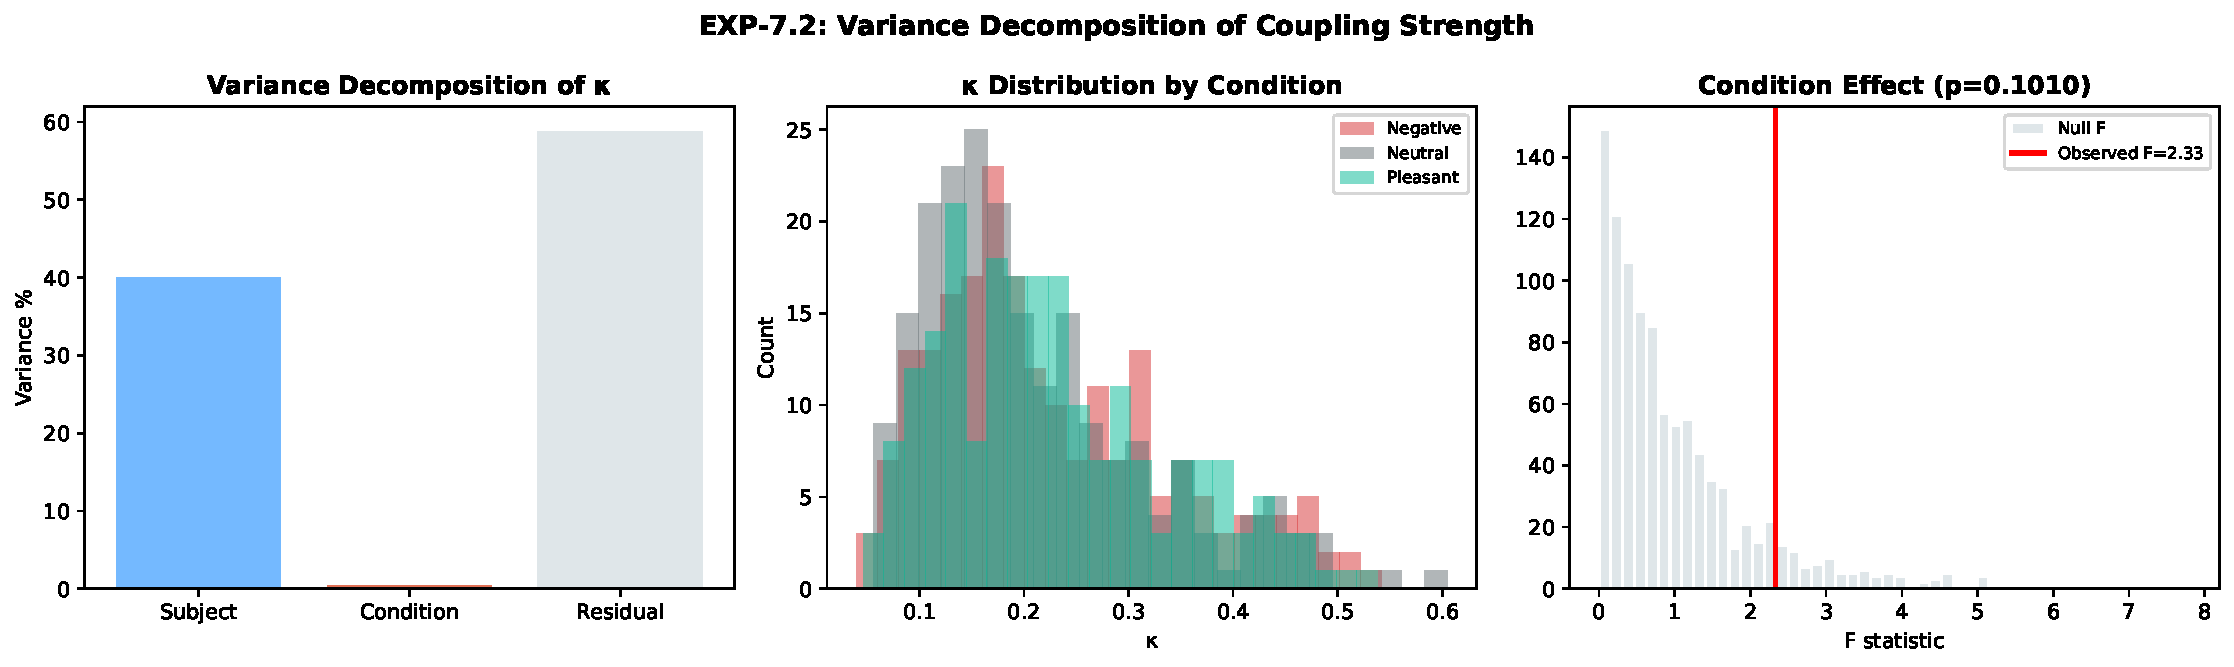
\includegraphics[width=\textwidth]{pictures/chSynthesis/fig_3class_variance_decomposition.pdf}
    \caption{Three-condition sample sums-of-squares decomposition: subject 40.3\%, condition 0.7\%, residual 59.0\%; condition permutation $p=0.101$. Fractions are descriptive and are not directly comparable with the unmatched four-category pipeline.}
    \label{fig:ch7_3class_variance}
\end{figure}

\subsection{Clinical Coupling at Three-Class}

No tested group comparison has $p<0.39$ in the three-condition analysis (Figure~\ref{fig:ch7_3class_clinical}); sample $d$ ranges from $-0.175$ to $+0.099$. This is lack of detected separation, not equivalence or evidence about independent clinical utility.

\begin{figure}[H]
    \centering
    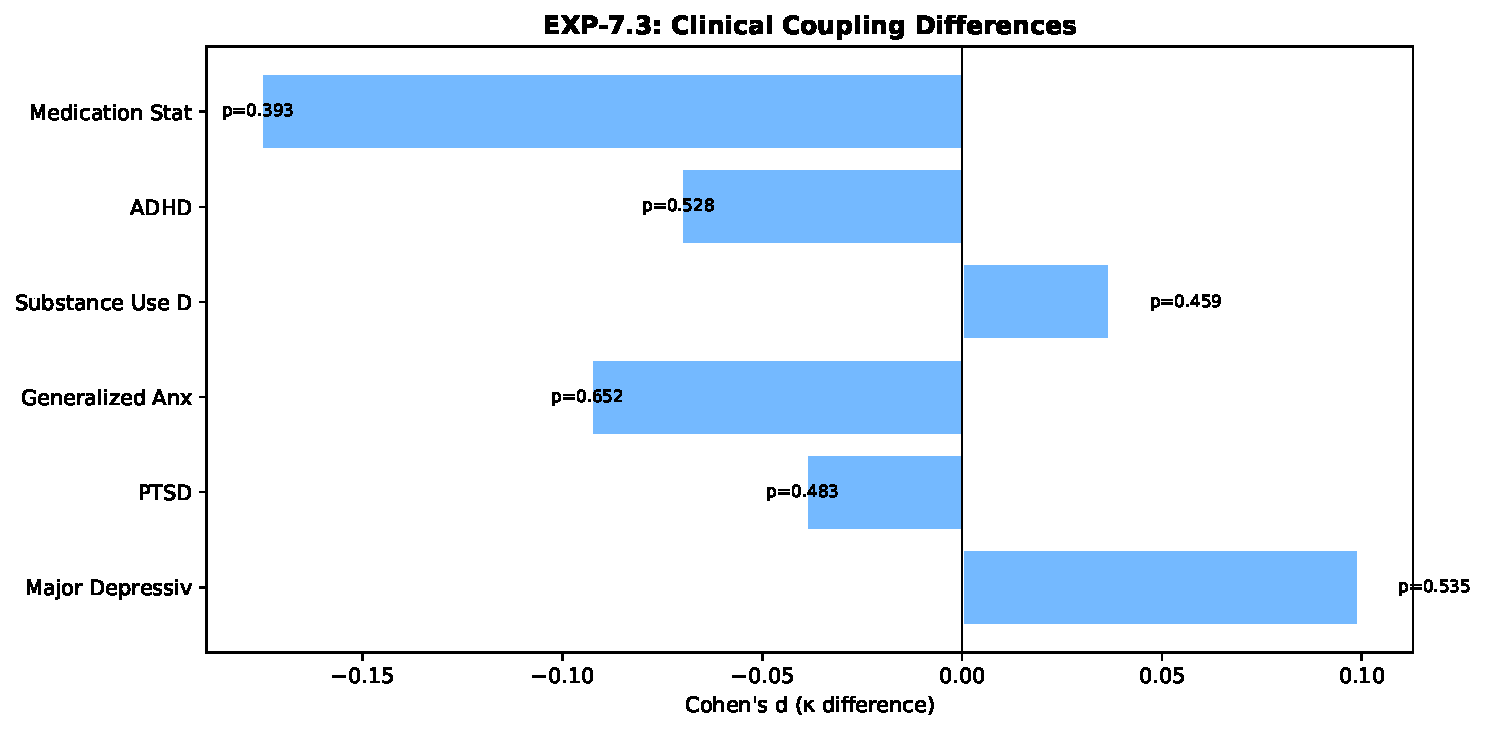
\includegraphics[width=0.85\textwidth]{pictures/chSynthesis/fig_3class_clinical_coupling.pdf}
    \caption{Three-condition coupling group comparisons for six clinical variables. No reported comparison has $p<0.39$; this does not establish equivalence.}
    \label{fig:ch7_3class_clinical}
\end{figure}

\subsection{Condition-Conditioned Coupling Structure at Three-Class}

The Frobenius norm test for pattern-level Negative--Pleasant differences in the coupling matrix produces $p = 0.376$, and zero of $14$ individual cells reach Bonferroni significance (Figure~\ref{fig:ch7_3class_condition}). The analysis therefore provides no evidence of a Negative--Pleasant pattern difference under the stated tests.

The Negative--Pleasant Frobenius test is non-significant, and the four-category Cute--Erotic scalar comparison is nominal and uncorrected while its pattern test is also non-significant. These results do not show that reorganization requires finer affective distinctions.

\begin{figure}[H]
    \centering
    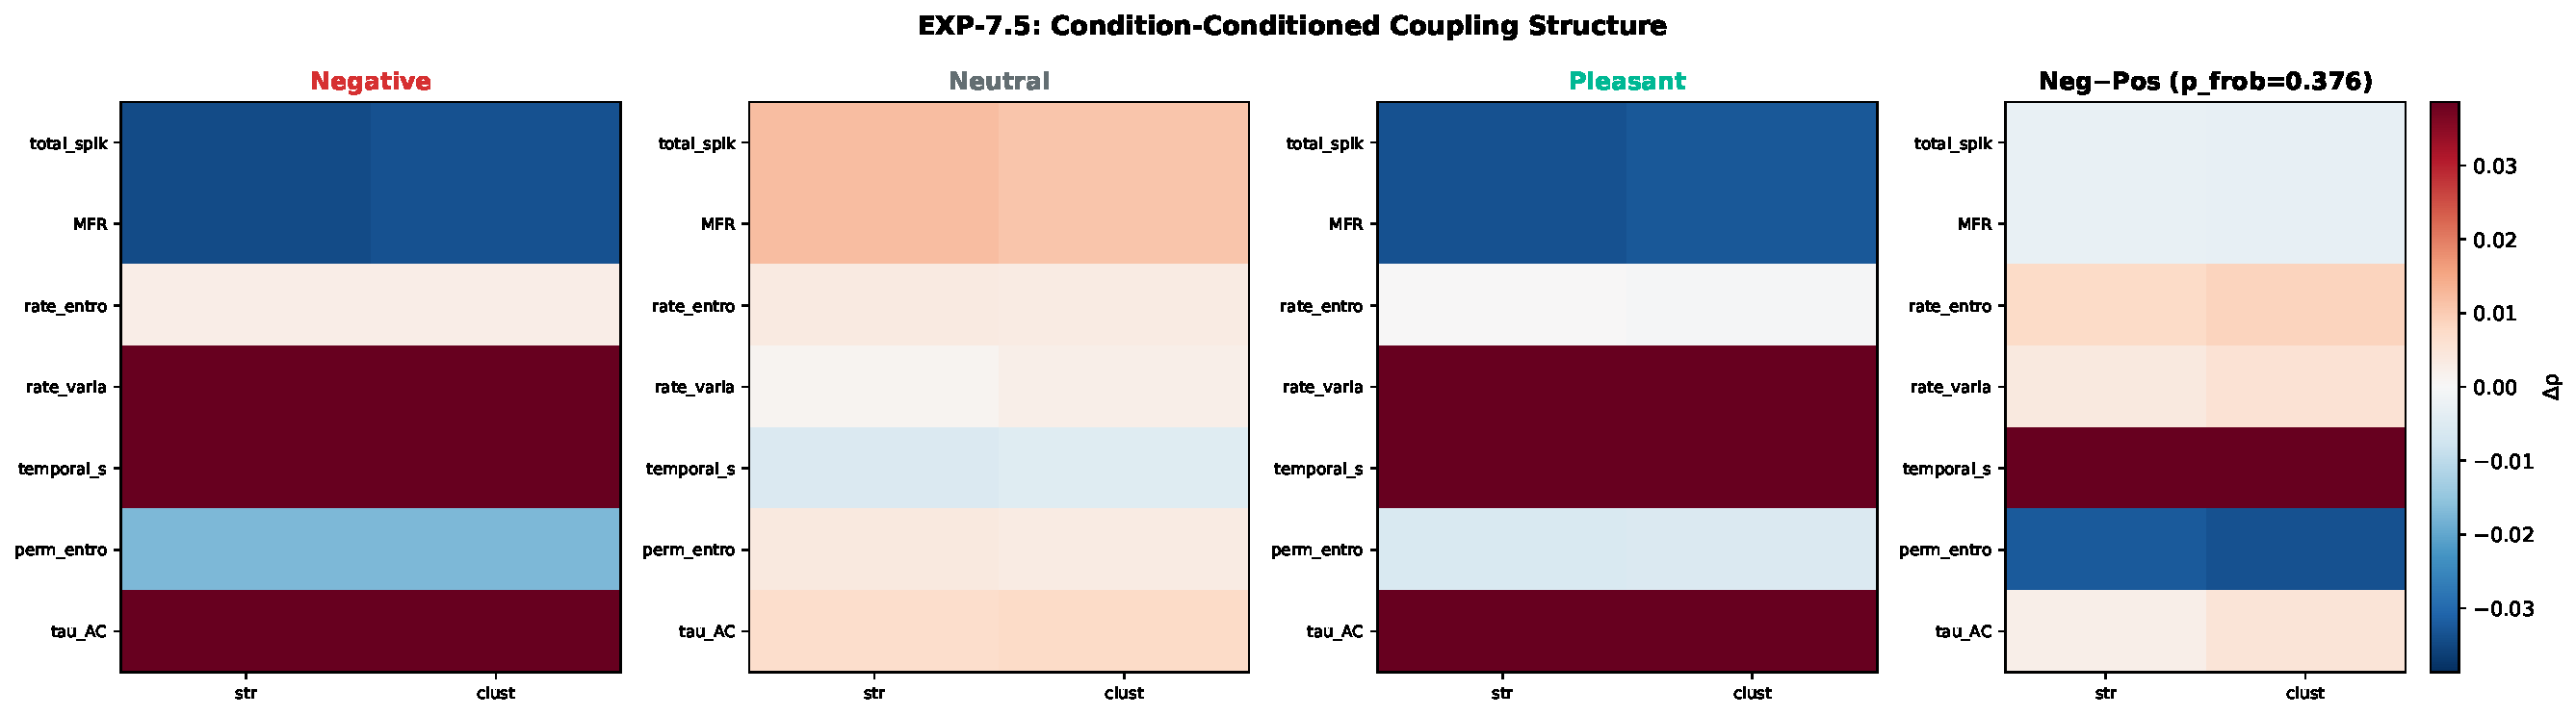
\includegraphics[width=\textwidth]{pictures/chSynthesis/fig_3class_condition_coupling.pdf}
    \caption{Three-condition coupling matrices and Negative--Pleasant difference matrix; the Frobenius sign-flip test gives $p=0.376$, with zero of 14 cells surviving Bonferroni correction.}
    \label{fig:ch7_3class_condition}
\end{figure}

\subsection{Augmentation Ablation at Three-Class}

In one fixed five-fold split, combined features do not exceed the better single family for the tested labels (Figure~\ref{fig:ch7_3class_augmentation}); balanced accuracies range from 43\% to 53\%. The invalid four-category fold-level $p$-value is not used, and the unmatched pipelines do not support a replication claim.

\begin{figure}[H]
    \centering
    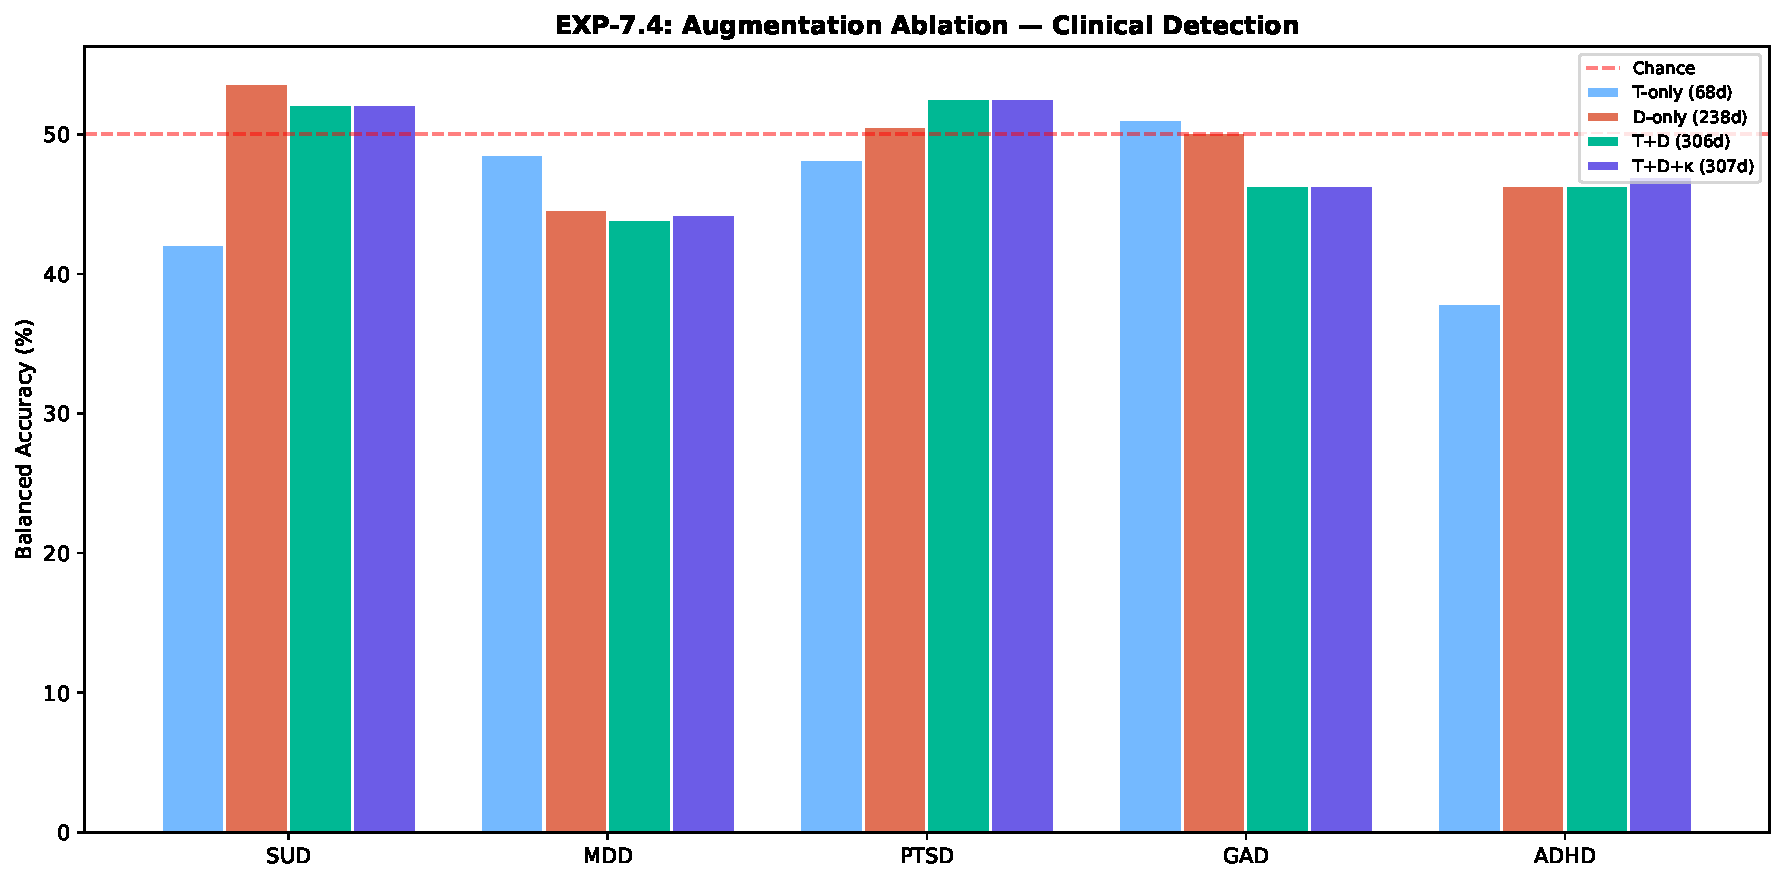
\includegraphics[width=0.85\textwidth]{pictures/chSynthesis/fig_3class_augmentation.pdf}
    \caption{Three-condition, fixed five-fold balanced accuracy for topology, dynamics, their concatenation, and concatenation plus $\kappa$. The finite comparison does not establish absence of complementary information.}
    \label{fig:ch7_3class_augmentation}
\end{figure}

\subsection{Cross-Granularity Summary}

Table~\ref{tab:ch7_cross_granularity} summarizes the coupling results across both granularities.

\begin{table}[H]
\centering
\caption{Descriptive comparison of unmatched three-condition and four-category pipelines.}
\label{tab:ch7_cross_granularity}
\footnotesize
\begin{tabularx}{\textwidth}{>{\raggedright\arraybackslash}p{3.2cm}>{\raggedright\arraybackslash}X>{\raggedright\arraybackslash}X}
\hline
\textbf{Property} & \textbf{3-class} & \textbf{4-class} \\
\hline
Mean $\kappa$ & $0.221$ & $0.290$ \\
Permutation summary & $1/5001\approx0.0002$ & Row-level paired $p=5.0\times10^{-113}$ (dependent rows) \\
Coupling direction & Mixed ($6/14$ negative) & Uniform (all negative) \\
Subject variance & $40.3\%$ & $29.2\%$ \\
Condition variance & $0.7\%$ ($p = 0.101$) & $0.6\%$ ($p = 0.133$) \\
Residual variance & $59.0\%$ & $70.1\%$ \\
Clinical $\kappa$ differences & None significant & None significant \\
Condition comparison & Frobenius $p=0.376$ & Cute--Erotic scalar $p=0.025$ uncorrected; Frobenius $p=0.177$ \\
Augmentation result & No sample-mean gain & ADHD D-only AUC 0.622; no valid fold-level $p$ \\
\hline
\end{tabularx}
\end{table}

Both pipelines show an observed mean coupling norm above their stated channel-shuffle null summaries, but only the three-condition pipeline has a coherent global Monte Carlo test. Sign, variance fractions, and clinical readout maxima differ across pipelines; because implementations are unmatched, those differences cannot be assigned to affective granularity.


\section{Chapter Synthesis}
\label{sec:ch7_synthesis}

Across the reported analyses, $\kappa$ provides a numerical summary of cross-channel association between two derived descriptor families. The audit narrows the inferential claims attached to that summary.

The three-condition mean exceeds its channel-shuffle null with corrected Monte Carlo $p\approx0.0002$. The four-category row-level results also show a descriptive shift, but dependency and legacy implementation differences prevent a confirmatory cross-pipeline claim. Residual sums of squares are large in both decompositions, but no test--retest data are available to determine trait stability.

No corrected clinical group comparison detects a $\kappa$ difference. Given limited power, comorbidity, and exploratory model selection, this is not evidence of equivalence or disorder specificity. Concatenation did not improve sample-mean performance in the recorded linear-readout comparisons.

The nominal Cute--Erotic scalar comparison and ADHD observations do not survive the relevant inferential checks and are not replications. They may motivate prespecified external testing, but they do not support a current clinical claim.

\subsection{The Three-Layer Architecture: An Integrated View}

For audit purposes, the pipeline can be divided into three computational layers. This organization records where quantities are produced; it does not establish that the layers are physiologically distinct or intrinsically interpretable:
\begin{enumerate}
    \item The \textbf{embedding layer} applies BSC$_6$ and PCA-64. Its archived real-data accuracies are descriptive legacy estimates because PCA and subject-centering procedures were not inductively evaluated.
    \item The \textbf{dynamical layer} computes seven named trajectory summaries. Their equations are inspectable, but several have arbitrary simulation units and no one-to-one mapping to ERP components.
    \item The \textbf{topology/coupling layer} computes within-epoch phase concentration, graph summaries, and $\kappa$. Reported clinical associations are nominal, uncorrected, or not permutation-significant.
\end{enumerate}
Post-hoc maxima differ by label and layer, but they do not establish disorder-specific sensitivity.

\subsection{Exploratory Prototype and Cross-Summary Descriptions}
\label{sec:ch7_level4}

The following prototype summaries were computed on the same cohort and are descriptive. They do not constitute a fourth level of validated interpretability, and the coupling audit above does not establish trait status.

The archived readout used 15 fitted prototypes. The mean within-subject agreement across three condition assignments is 0.48. Without a permutation baseline, repeated-session data, or an external fit/evaluation split for the prototype analysis, this value does not separate condition dependence from instability or overfitting.

Across 211 subjects, same-prototype proportions are 28\% for Negative--Pleasant, 35\% for Negative--Neutral, and 33\% for Pleasant--Neutral. No inferential comparison is reported, so these percentages are not evidence of a recovered affective geometry.

Neutral-dominant Prototypes~9 (93\% purity, $n=27$) and~5 (74\% purity, $n=90$) have different sample P300 summaries. This does not establish stable subtypes or an advantage over a flat classifier without a prespecified, held-out comparison.

Mapping 15 binary clinical variables onto dominant prototype assignments produces many small-cell prevalence comparisons. Three selected examples are:
\begin{itemize}
    \item \textbf{Prototype~4} (Negative-dominant, $n=5$): PDD 80\% versus 37\% in the cohort, PTSD 60\% versus 40\%, and recurrent MDD 80\% versus 57\%.
    \item \textbf{Prototype~8} (Neutral-dominant, $n=27$): GAD 46\% versus 29\%, PTSD 27\% versus 40\%, and eating disorders 23\% versus 33\%.
    \item \textbf{Prototype~13} (Pleasant-dominant, $n=12$): MDD 91\% versus 69\%, PTSD 18\% versus 40\%, and GAD 9\% versus 29\%.
\end{itemize}
These examples were selected after inspecting many prototype--diagnosis cells, some with $n=5$. No diagnosis--prototype test has $p<0.05$ (all $p>0.07$, Cram\'{e}r's $V<0.16$), even before a clearly defined family-wise correction. The profiles do not establish patient subgroups or subtypes.

Condition assignments, prototype purity, transition counts, ERP summaries, and $\kappa$ offer several cohort descriptions. Their reliability and patient-level validity were not tested. The appropriate claim is inspectability of the calculations, not completion of a validated interpretability chain.

The methodological contribution is the explicit definition of a channel-wise coupling summary within this pipeline. Comparisons with prototype, graph, or attribution methods in other systems are conceptual because they operate on different data and targets \cite{barnett_protopmed_2024,kasabov_neucube_2014}.

\subsection{Scope and Future Directions}

Future work should use single-trial data, a labeled montage, repeated sessions, common preprocessing across condition schemes, and prespecified frequency-band and graph-construction sensitivity analyses. Clinical studies should use externally fitted models, comorbidity-aware designs, and dimensional outcomes. Sample size should be determined prospectively from an independent effect estimate rather than the selected uncorrected cells reported here.
